\documentclass[preprint,12pt]{elsarticle}
\usepackage{amssymb}
\usepackage{amsmath}
\usepackage[hidelinks]{hyperref}
\usepackage[acronym]{glossaries} % load gói glossaries
\makeglossaries
\newacronym{pdp}{PDP}{pickup and delivery problem}
\newacronym{vrp}{VRP}{vehicle routing problem}
\newacronym{dpdp}{DPDP}{dynamic pickup and delivery problem}
\newacronym{pdptw}{PDPTW}{pickup and delivery problem with time windows}
\newacronym{aglisa}{AGVNS}{adaptive genetic and variable neighborhood search algorithm}
\newacronym{vns}{VNS}{variable neighborhood search}
\newacronym{gas}{GAs}{genetic algorithms}
\newacronym{ga}{GA}{genetic algorithm}
\newacronym{ma}{MA}{memetic algorithm}

\newacronym{vnsme}{VNSME}{variable neighborhood search with multiple local search strategies and efficient disturbance}
\newacronym{im}{IM}{insertion method}
\newacronym{ls}{LS}{local search}
\newacronym{ts}{TS}{tabu search}

\usepackage{longtable}
\usepackage{graphicx}
\usepackage[utf8]{inputenc}
\usepackage{xcolor}
\usepackage{pgfplotstable}
\usepackage{hyperref}
\usepackage{multirow} 
\usepackage{booktabs}
\usepackage{subcaption}
\usepackage{longtable}
\usepackage{amsmath}
\usepackage{lipsum, multicol}
\usepackage{makecell}
\usepackage[numbers]{natbib}
\usepackage{float}
\usepackage{caption}
\usepackage{mathtools}
\usepackage{comment}
\usepackage{placeins}
\usepackage{graphicx}
\usepackage{amsmath,amssymb}
\usepackage{mathtools}
\usepackage{xcolor}
\usepackage{color}
\usepackage{threeparttable}
\usepackage{tabularx}
\usepackage{amsmath}
\usepackage[linesnumbered,ruled,vlined]{algorithm2e}


\begin{document}
\begin{frontmatter}
\title{	
Adaptive Hybrid Evolutionary Search for Dynamic Pickup and Delivery Problems with Time Windows}
\author[1]{Tran Dinh Phuc} \ead{phuc.td224891@sis.hust.edu.vn} 
        \author[2]{Nguyen Thi Tam \corref{cor1}}\ead{tamnt@vnu.edu.vn}
		\author[1]{Huynh Thi Thanh Binh} \ead{binhht@soict.hust.edu.vn}
		\cortext[cor1]{Corresponding author}
		\affiliation[1]{
			organization={Hanoi University of Science and Technology}, 
			state={Hanoi}, 
			country={Vietnam}
		}
		\affiliation[2]{
			organization={VNU University of Science}, 
			state={Hanoi}, 
			country={Vietnam}
		}

\begin{abstract}
The dynamic pickup and delivery problem (DPDP) is a fundamental challenge in modern logistics systems, where customer requests arrive continuously over time and require real-time routing decisions. In this study, we investigate a practical DPDP motivated by real-world delivery operations at Huawei, characterized by stochastic order arrivals and strict time window constraints. To effectively address the dynamic and large-scale nature of the problem, we propose an adaptive hybrid optimization framework, namely Adaptive Genetic Variable Neighborhood Search (AGVNS), which combines global exploration capabilities of genetic algorithms with adaptive local refinement through variable neighborhood search.
Unlike conventional approaches that rely on static or periodically updated solutions, the proposed method dynamically re-optimizes routing decisions in response to newly arriving requests, enabling a better balance between exploration and exploitation during the search process. In addition, an adaptive mechanism is introduced to adjust search behaviors based on the evolving state of the system, enhancing both solution quality and robustness.
Extensive computational experiments on 64 real-world instances demonstrate that the proposed AGVNS consistently outperforms several competitive state-of-the-art algorithms in terms of total operational cost and solution stability. The results highlight the effectiveness of the proposed approach in handling large-scale dynamic pickup and delivery problems with time windows, and its potential for real-world logistics applications.
\end{abstract}


\begin{keyword}
dynamic pickup and delivery problem, local search, genetic algorithm
\end{keyword}

\end{frontmatter}

\section{Introduction}\label{sec1}

The \gls{vrp} is one of the most fundamental and widely studied combinatorial optimization problems in transportation and logistics \cite{toth2002vehicle}. It aims to determine an optimal set of routes for a fleet of vehicles to serve a group of customers with known demands while optimizing the total travel costs. Over the decades, \gls{vrp} and its variants  have played an important role in modern logistics optimization, enabling efficient distribution, fleet management, and resource allocation in various industries. 

However, in many real-world applications, such as courier delivery and ride-sharing, transportation requests are not only about visiting customers but also involve picking up and delivering items. This gives rise to \gls{pdp}, a more complex variant of the \gls{vrp} that incorporates priority constraints between pickup and delivery locations, as well as vehicle capacity and time window constraints \cite{savelsbergh1995general}. The \gls{pdp} better reflects the operational characteristics of modern logistics systems.

While static \gls{pdp} assumes that all requests are known in advance, this assumption rarely holds in practical, real-time environments \cite{, jeong2024dynamic, wang2025multi, xiang2024centralized, zhou2024pickup}. In many  logistics operations, transportation requests usually arrive dynamically over time. Such situations lead to the \gls{dpdp}, where the routing plan must be continuously updated in response to new requests. The \gls{dpdp} investigated in this study is formulated based on the  International Conference on Automated Planning and Scheduling in 2021 (ICAPS 2021)  challenge problem \cite{hao2022introduction}. The competition focuses on optimizing dynamic logistics operations where requests continuously appear during execution, vehicles have limited capacities, and service time windows must be respected. The ICAP benchmark provides a realistic and large-scale testbed that captures the stochastic and dynamic nature of real-world delivery systems, making it an ideal platform to evaluate algorithms. 

The static routing algorithms struggle in dynamic environments due to their limited adaptability and computational efficiency. Due to the dynamic nature of the problem, where new requests frequently arise, the algorithm must provide rapid responses. Designing an algorithm that balances solution quality and computational speed in such a setting remains an open and challenging research question.

Despite the extensive research on pickup and delivery problems and their dynamic variants, most existing solution approaches rely primarily on a single metaheuristic framework, such as \gls{vns} or evolutionary algorithms \cite{horvath2025recent, voigt2025review}. While these methods have achieved notable success in various problem settings, they exhibit inherent limitations when applied to large-scale, highly dynamic logistics environments. \gls{vns}-based methods are effective in performing local search and exploring multiple neighborhood structures to improve solution quality. However, they often lack global exploration capability, which can lead to local optima. Conversely,the evolutionary algorithm such as \gls{gas} offer strong global search capabilities through population-based evolution, but they may converge slowly and struggle to adjust solutions without additional local search mechanisms \cite{cai2024decomposition, wang2024hybrid}.

To address these challenges, we propose an adaptive genetic and variable neighborhood search algorithm that combines the global exploration ability of genetic algorithms with the intensive exploitation capability of local search. The proposed algorithm dynamically adjusts evolutionary parameters, such as the crossover probability based on real-time performance feedback of the search process. Additionally, a local search module is integrated to adjust promising solutions and enhance convergence toward high-quality routing plans. This hybrid adaptive mechanism enables the algorithm to effectively respond to dynamic changes while maintaining computational efficiency. We conduct extensive experiments on the ICAP 2021 benchmark datasets, demonstrating that our proposed method consistently outperforms baseline approaches in terms of solution quality, adaptability, and computational efficiency.


The remainder of this paper is organized as follows. Section \ref{sec:problem} presents the formal problem definition and mathematical formulation. Section \ref{sec:related} reviews the existing literature on the ICAPS-DPDP.
Section \ref{sec:proposed} introduces the proposed adaptive genetic and local search algorithm in detail. Section \ref{sec:exp} reports the experimental setup, benchmark results, and comparative analysis. Finally, Section \ref{sec:con} concludes the paper and outlines potential directions for future research.

\section{Problem formulation}\label{sec:problem} 

Our study considers a special variant of the ICAPS-DPDP, a central challenge in modern logistics. The problem involves dynamically assigning and routing a fleet of vehicles to serve customer requests that appear over time, while accounting for several real-world operational constraints. Specifically, vehicle capacities, time windows, loading rules, and limited docking facilities introduce complex interdependencies that directly affect service performance. Unlike traditional models, our formulation captures these operational realities with the goal of optimizing fleet routes to balance delivery delays and travel distance. To formally describe this problem, we outline its main components: input, output, constraints, and objectives.

\textbf{Input}

The comprehensive set of input data is described by three key components, including the route network, the order set, and the vehicle fleet, together with all associated operational constraints.

Firstly, the operational environment is modeled as a complete directed graph, $\textbf{G = (F, A)}$, which represents a closed-loop logistics network. 
\begin{itemize}
    \item The set of nodes, $\textbf{F} = \{F^i | i = 1, \dots, M\}$, in which $F^i$ denotes the $i$-th factory in the set and there are $M$ distinct factories that serve as the central hubs for all pickup and delivery operations.
    
    \item The arc set, $\textbf{A} = \{(i, j) | i, j \in M, i \neq j\}$, contains all possible directed transportation links between any two factories. Each arc is characterized by two essential attributes: a static transportation distance ($d_{ij}$) and a corresponding transportation time ($t_{ij}$). These parameters form the fundamental cost structure for all vehicle movements.

    \item Furthermore, the model incorporates critical constraints at the factory level. Each factory has a fixed, limited number of cargo docks for loading and unloading $\textbf{D} = \{ D^i \mid i \in [1 , \dots , M]\}$. A fixed dock approaching time $DAT$ is allocated for a vehicle to move from its arrival point to an assigned dock, a necessary step independent of any queuing delay.

\end{itemize}

Secondly, the system's demand is specified by a dynamic set of orders, $\textbf{O} = \{o^i | i = 1, \dots, N\}$, that are introduced into the system randomly over time. Each order is defined by a tuple $(F_{p}^i, F_{d}^i, q^i, t_{e}^i, t_{l}^i)$ containing critical details:
\begin{itemize}
    \item Pickup and Delivery Locations: $F_{p}^i$ and $F_{d}^i$ are the specific factory nodes where cargo must be picked up and delivered.
    
    \item Cargo Volume: The cargo amount, $q^i$, is represented by a multi-unit vector $q^i = (q_{standard}^i, q_{small}^i, q_{box}^i)$, accounting for different unit types with conversions: 1 standard pallet = 2 small pallets = 4 boxes. This multi-unit representation is crucial for accurately calculating vehicle capacity and handling times. The time required for loading ($t_p^i$) and unloading ($t_d^i$) is directly proportional to the number of each type of pallet. It is calculated as:
\begin{equation}
t_p^i = t_d^i = \omega_{standard} \times q_{standard}^i 
+ \omega_{small} \times q_{small}^i 
+ \omega_{box} \times q_{box}^i
\end{equation}
    with $\omega$ seconds per corresponding type supply. 
    
    \item Time window: Each order has a creation time ($t_{e}^i$) and a strict committed completion time ($t_{l}^i$), which serves as an all-inclusive deadline for the entire fulfillment process.
\end{itemize}

Finally, the transportation service is provided by a homogeneous fleet of $K$ vehicles, denoted $\textbf{V} = \{v^k | k = 1, \dots, K\}$. Each vehicle has a uniform loading capacity $Q$. Their initial positions are randomly assigned to a factory node, reflecting a flexible dispatch system. 

\textbf{Output}

The output of the model is a comprehensive solution, denoted by $\textbf{R} = \{r^k | k = 1, \dots, K\}$. This solution comprises a detailed assignment and routing plan for each vehicle in the fleet. Each $r^k$ represents the planned route for vehicle $k$, which is a consecutive sequence of factory visits required to fulfill its assigned orders. We denote the route of the $k$-th vehicle as $r^k = \{m_1^k, m_2^k, \dots, m_{l_k}^k\}$, where $l_k$ is the total number of visits on that route, and $m_j^k$ is the $j$-th factory node visited by vehicle $k$. The final output provides a complete operational schedule, including the specific sequence of pickups and deliveries for each vehicle, ensuring that all orders are serviced.

\textbf{Objectives}

The first objective, overtime penalty ($OVP$), focuses on timely delivery of orders. It is designed to penalize any delay beyond an order's committed completion time. This objective is defined as the sum of all individual order timeouts:

\begin{equation}
OVP = \sum_{i=1}^{N} \max(0, a_d^i - t_l^i)
\end{equation}

where $N$ is the total number of orders, $a_d^i$ is the arrival time of the order $o^i$ at its destination node. The $\max(0, \cdot)$ function ensures that only delays (where $a_d^i > t_l^i$) contribute to the total timeout cost, while on-time or early deliveries do not incur any penalty.

The second objective, average traveling distance ($ATD$), aims to minimize the operational costs associated with vehicle travel. It is represented by the average travel distance across the entire fleet. This objective is formulated as follows:

\begin{equation}
ATD = \frac{1}{K} \sum_{k=1}^{K} \sum_{i=1}^{l_k - 1} d_{m_i^k, m_{i+1}^k}
\end{equation}

where $K$ is the total number of vehicles in the fleet. The route plan of vehicle $v^k$ is given by the sequence of visited nodes, $r^k = \{m_1^k, m_2^k, \dots, m_{l_k}^k\}$. The inner sum calculates the total distance traveled by vehicle $k$, with $d_{m_i^k, m_{i+1}^k}$ being the distance from node $m_i^k$ to node $m_{i+1}^k$. Dividing by $K$ provides the average distance, promoting a balanced and efficient utilization of the fleet.

The final objective is a combination of the two sub-objectives, formulated to prioritize the time-sensitive nature of the problem. The overall function $f$ is given by:

\begin{equation}\label{eq:f}
f = \lambda \times OVP + ATD    
\end{equation}

In this formulation, $\lambda$ is a large positive constant. The use of a large $\lambda$ value ensures that minimizing the total timeout ($OVP$) is given significantly higher priority than minimizing the average travel distance ($ATD$). This weighting scheme reflects the business reality where meeting delivery deadlines is paramount, while travel distance optimization serves as a secondary concern to improve overall efficiency without compromising service quality. This formulation guides the optimization algorithm to find a solution that first and foremost prevents late deliveries before seeking to reduce operational costs.

\textbf{Constraints}

The proposed model operates under a series of real-world constraints that govern the feasibility of any given solution. These constraints are categorized to ensure that the routing and scheduling plan is both practical and robust.

\begin{enumerate}
    \item A fundamental requirement of our model is that every order in the set $\textbf{O}$ must be fulfilled. To ensure this, each order must be assigned to exactly one vehicle from the fleet $\textbf{V}$. This assignment is defined by an assignment matrix $\textbf{y}$, where the binary variable $y_{ik}$ takes the value of 1 if vehicle $k$ is assigned to serve order $i$, and 0 otherwise. This matrix is a key component of the overall problem formulation.

\begin{equation}
    \sum_{k=1}^K y_{ik} = 1, \quad \forall i \in [1, \dots , N]
\end{equation}
    
    \item Each order $o^i$ is associated with a committed completion time, $t_l^i$. While the model's primary goal is to respect this deadline, the constraint is considered a soft constraint. This implies that an order's delivery arrival time, $a_d^i$, may exceed $t_l^i$, but any resulting timeout will contribute to the total penalty component of the objective function. 

\begin{equation}
    t_e ^i \leq a_d^i \leq t_l^i, \quad \forall i \in [1 , \dots,  N]
\end{equation}

    \item Order splitting is exclusively allowed for orders whose total volume surpasses a single vehicle's loading capacity. A critical constraint of this process is that the smallest units of cargo - a standard pallet, a small pallet, or a box—are not divisible. Therefore, these items cannot be split into their smaller constituent units (e.g., a standard pallet cannot be divided into two small pallets). In the dispatching phase, we operate on the assumption that any necessary order splitting has been preprocessed, and we deal directly with the resulting suborders, denoted as $o^i_h$. Each original order $o^i$ is thus assumed to have been partitioned into a set of $\mathcal{H} ^i$ suborders. The total demand for any given order $o^i$ is calculated using the following function:

\begin{equation}
    \text{demand}(o^i) = q^i_{\text{standard}} + \frac{1}{2} q^i_{\text{small}} + \frac{1}{4} q^i_{\text{boxes}}
\end{equation}

\begin{equation}
     \text{demand}(o^i) = \sum_{h = 1}^{ \mathcal{H} ^i} \text{demand}(o^i_h)
\end{equation}

\begin{equation}
     0 < \text{demand}(o^i_h) \leq Q , \quad \forall h\in [1 , \dots , \mathcal{H}^i] , \quad \forall i \in [1, \dots , N] 
\end{equation}


    \item Another key constraint is that the total cargo volume carried by any vehicle must not exceed its maximum loading capacity, $Q$. For each vehicle $v_k$, we use the continuous variable $Q^k_{m_i^k , m_{i+1}^k}$ to represent its current load as it travels between consecutive nodes $m_i^k$ and $m_{i+1}^k$ on its planned route. This variable ensures that the capacity constraint is met at all times throughout the journey, as formally expressed by:

\begin{equation}
    Q^k_{m_i^k , m_{i +1}^k} \leq Q , \quad \forall i \in [1 , \dots , l_k - 1] , \quad \forall k \in [1, \dots , K]
\end{equation}

    \item The Last-In, First-Out (LIFO) loading constraint is a crucial operational rule that ensures items can be unloaded from a vehicle without having to rearrange other cargo. For any two orders, $o_i$ and $o_j$, assigned to the same vehicle, if order $i$ is picked up before order $j$, then order $j$ must be delivered before order $i$. This is because the last item loaded is the first to be accessible for unloading. We utilize the binary variable $z_{ij} \in \{0,1\}$, which is equal to 1 if order $i$ is picked up before order $j$ by the same vehicle. 
\begin{equation}
  (a_{d}^j - a_{d}^i) \leq \mathcal{M}(1 - z_{ij}) - \epsilon, \quad \forall i, j \in [1 , \dots , N], i \neq j   
\end{equation}
where $\epsilon$ is a small positive value (e.g., 0.001) to enforce a strict inequality and $\mathcal{M}$ is a very large positive constant.

    \item Each factory node $F^i$ has a limited number of cargo docks. The number of vehicles being serviced at a factory at any time cannot exceed this capacity. This can be expressed as:
\begin{equation}
    \sum_{k = 1}^K u_{i k} \leq D^i, \quad \forall i \in [1 , \dots , M]
\end{equation}
where $ u_{i k} \in \{0 , 1\}$ determine whether vehicles $k$ being serviced at factory $F^i$.

    \item The allocation of docks follows a First-Come, First-Served (FCFS) rule. This means that vehicles are serviced in the order of their arrival. In a simulated environment, random selection might be necessary for simultaneous arrivals, but the core principle is that a vehicle's service cannot begin until all preceding vehicles in the queue have been serviced. The service start time for vehicle $k$ at factory $i$ is thus a function of the completion times of other vehicles being serviced or waiting at that facility.
    
\end{enumerate}

In summary, the above constraints collectively ensure that the routing and scheduling plan remains feasible and operationally consistent at all times. They cover assignment, timing, capacity, loading rules, and docking limitations, which together capture the key practical aspects of the problem. By enforcing these conditions throughout the planning horizon, the model guarantees that any solution is both implementable in practice and aligned with real-world logistics requirements.

%\section{Related work on the ICAPS dynamic pickup and delivery problem}
\section{Related work}\label{sec:related}
\subsection{Algorithms from the ICAPS 2021 DPDP Competition}
\subsubsection{Variable neighborhood search}
The gold-prize-winning algorithm of the ICAPS 2021 DPDP competition, referred to as \gls{vnsme} \cite{cai2022variable}, represents one of the most effective algorithm frameworks designed for real-time logistics optimization. The competition problem models a realistic dynamic environment where new pickup and delivery requests arrive over time, and routing decisions must be updated efficiently under strict time and capacity constraints. The \gls{vnsme} algorithm extends the \gls{vns} with multiple local search strategies and an Efficient disturbance. In particular, the best solution from the previous iteration is reconstructed to form the initial solution for the current one using two heuristic procedures: an exhaustive reconstruction and a cheapest insertion strategy, which ensure feasibility and computational efficiency.

During each optimization phase, \gls{vnsme} employs four local search operators such as couple exchange, block-exchange, block relocate, and multi relocate to intensively explore the solution neighborhood. These operators cooperatively enhance solution efficiency by adjusting multiple routes and maintaining pickup–delivery precedence. To further prevent early convergence, the algorithm introduces an efficient disturbance mechanism based on a modified 2-opt-L operator, which introduces controlled perturbations for escaping local optima while preserving promising solution structures. The combined design allows VNSME to effectively balance exploration and exploitation, achieving high-quality solutions in a dynamic and computationally constrained environment. Experimental evaluations on the official Huawei DPDP benchmarks confirm its superior performance, where VNSME ranked first among 153 teams in the ICAPS 2021 DPDP competition.

Despite its remarkable performance, the algorithm exhibits certain limitations. Specifically, its stochastic nature makes the results non-deterministic across runs, and the selection of local search operators remains manually tuned. Moreover, the algorithm lacks an adaptive component to dynamically adjust search parameters according to problem evolution. These limitations highlight potential directions for improvement, particularly through the integration of evolutionary adaptation or reinforcement learning mechanisms—a motivation that inspires the approach proposed in this paper.
\subsubsection{Insertion method}
The \gls{im}, which won the silver prize in the ICAPS 2021 DPDP competition, employs a heuristic strategy to generate feasible routing plans at each decision period. When new customer requests are arrived, the algorithm integrates them into existing vehicle routes using an insertion cost function that jointly considers travel distance, service time feasibility, and vehicle capacity. By prioritizing minimal disruption to current routes, IM ensures that new orders are accommodated efficiently while maintaining feasibility with respect to all operational constraints, including time windows and vehicle load limits. Despite its algorithmic simplicity, IM demonstrates strong adaptability and computational efficiency, making it particularly well-suited for real-time dynamic routing environments where rapid response is critical
\subsubsection{Local search}

The \gls{ls} algorithm, which achieved the bronze prize in the ICAPS 2021 DPDP competition, designed based on the insertion-based framework but enhances it through an iterative local improvement mechanism inspired by the \gls{vns} algorithm. In each iteration, the algorithm begins by constructing an initial feasible solution using a two-phase insertion strategy. First, urgent orders—those with imminent time window deadlines—are prioritized and inserted into the current route plan to ensure timely service. Next, the remaining orders are incorporated based on their estimated travel time, with customers requiring longer trips being scheduled earlier to balance workload and minimize lateness risk.
By combining a heuristic construction phase with a focused improvement process, the \gls{ls} algorithm achieves a balance between computational efficiency and solution refinement. Its structured yet lightweight design allows it to adapt dynamically to incoming requests, making it an effective and competitive approach for real-time dynamic pickup and delivery operations. Its simple and flexible design helps it adjust quickly when new requests arrive, making it a useful and effective method for real-time pickup and delivery tasks.

\subsection{Other algorithms}
\label{sec:other_algo}
In \cite{zhou2024memetic}, the authors focus on a variant of the \gls{dpdp} with multiple practical constraints. The authors propose a memetic algorithm that combines a genetic algorithm for exploring the search space and a local search procedure for refining solutions in promising regions. This hybrid design effectively balances exploration and exploitation, leading to high-quality solutions. However, in the recent study \cite{horvath2025recent}, the authors critically re-examined the work of Zhou et al. and pointed out that their algorithm did not actually address the original ICAPS 2021 DPDP problem introduced in the Huawei 2021 competition. Instead, it was applied to a relaxed variant of the problem that omitted some essential constraints of the original formulation. Their reproducible computational experiments revealed that the original and relaxed versions differ significantly in both complexity and solution characteristics. Consequently, the results reported by Zhou et al. may not accurately reflect performance on the true ICAPS-DPDP. In this study, we reimplement and adapt the memetic algorithm proposed in \cite{zhou2024memetic} to ensure full compatibility with the original ICAPS-DPDP formulation. Necessary modifications are introduced to strictly enforce all problem constraints defined in the competition setting, thereby addressing the limitations identified in prior work. The adapted version serves as a baseline algorithm for fair and consistent comparison with our proposed method. This allows us to rigorously evaluate the effectiveness of our approach in solving the real-world dynamic pickup and delivery problem under realistic and dynamic conditions.

\section{Proposed methodology} \label{sec:proposed}

\begin{figure}
    \centering
    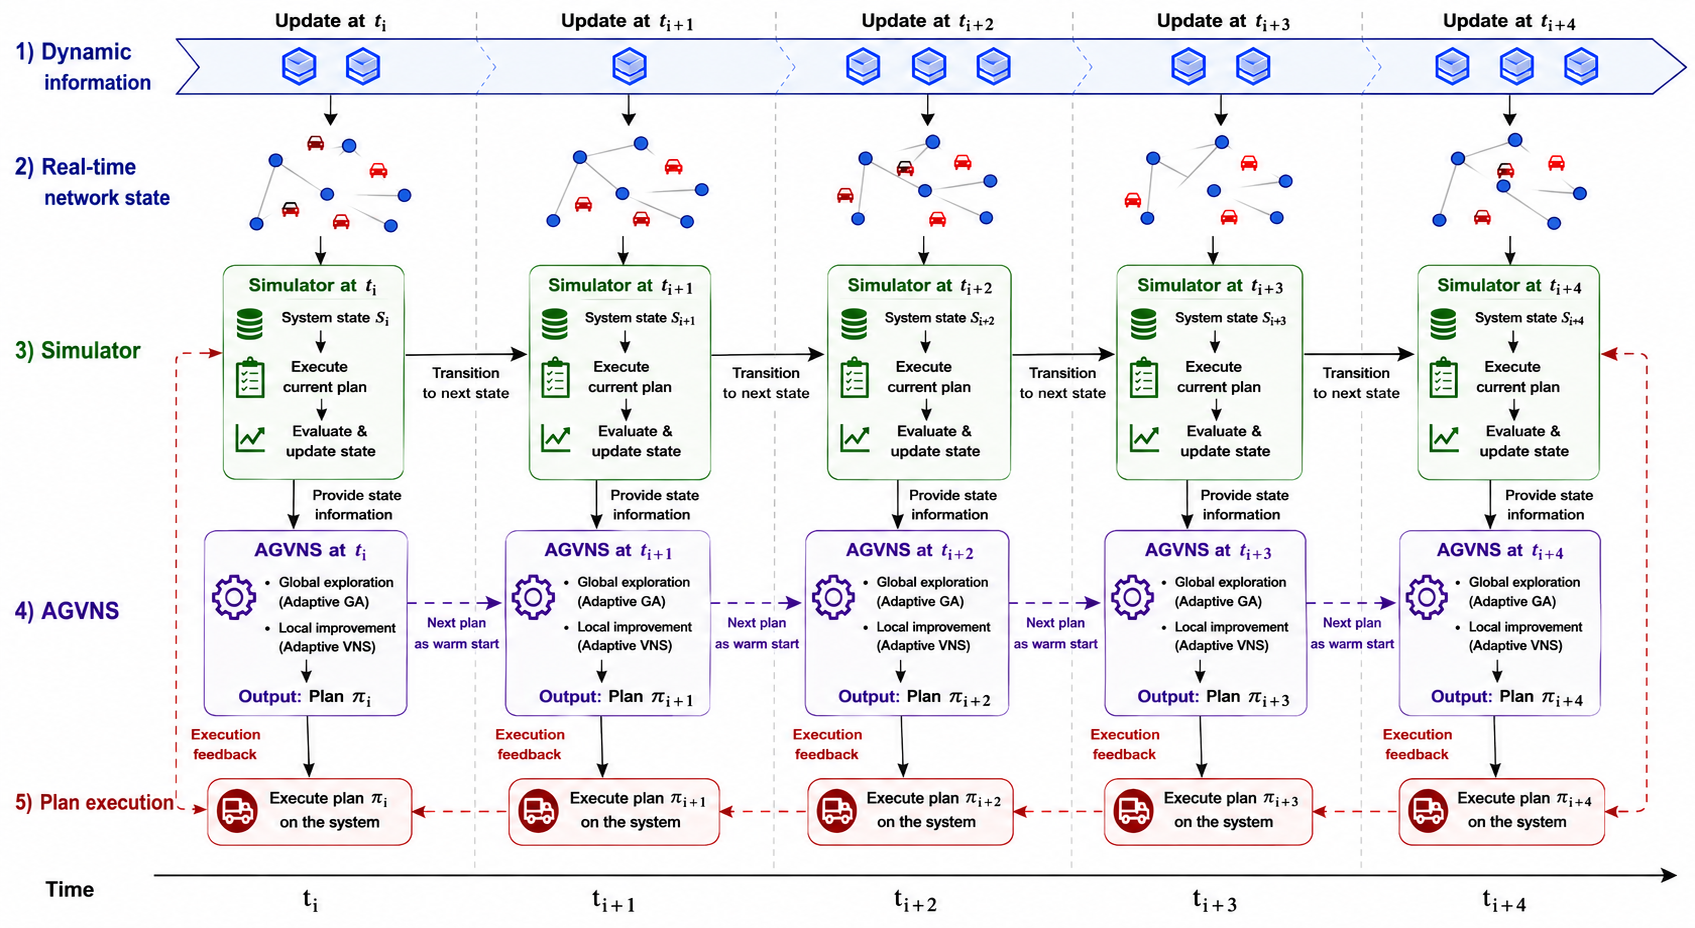
\includegraphics[width=0.85\linewidth]{figure/simulator.png}
    \caption{The illustration of the periodic re-optimization framework.}
    \label{fig:sequential_process}
\end{figure}


Our proposed methodology, called \gls{aglisa} addresses the \gls{dpdp} via a periodic re-optimization framework that decomposes the dynamic problem into a sequence of static \gls{pdp} subproblems at discrete time intervals. Each subproblem represents a relaxation of the original DPDP, incorporating updated inputs to enable the use of robust and efficient algorithms to generate high quality routing plans for a homogeneous vehicle fleet. At each predefined update point, the simulator gathers real-time system information, including newly released customer requests, pending deliveries, and current vehicle states, to form an accurate snapshot of the operational environment. The optimization module then computes a feasible, fleet-wide routing plan, which is executed until the next update, whereupon the cycle recommences with refreshed data. This iterative loop of simulation, information updating, and re-optimization ensures continuous adaptation to evolving demand and resource availability while maintaining a favorable trade-off between solution quality and computational efficiency. By employing proven static solvers within each time window, the framework maintains global consistency across successive decision stages and has proven effective in prior benchmarks, including the winning solution of the ICAPS 2021 competition~\cite{cai2022variable}.  

As illustrated in Figure~\ref{fig:sequential_process}, at discrete time instants \( t_i, t_{i+1}, t_{i+2}, t_{i+3}, t_{i+4} \), dynamic information (new requests, unserved orders, and vehicle states) is injected into the simulator. Each resulting snapshot defines a static PDP subproblem, which \gls{aglisa} solves to yield an updated routing configuration for the fleet. 
The derived plan is then implemented, yielding the subsequent update, while the unused portion of the current interval is skipped. This approach maintains a closed-loop process of simulation, optimization, and plan execution throughout the time horizon. The detailed components of the proposed framework are elaborated in the following sections.

%\subsection{Decomposition mechanism of the planning horizon}

% According to \cite{7743429}, methodologies for the Dynamic Vehicle Routing Problem (DVRP) are generally classified into three categories: (i) deterministic dynamic routing, which assumes certainty in new information and applies periodic or continuous re-optimization of static subproblems; (ii) stochastic dynamic routing, which incorporates probabilistic knowledge of future events through stochastic programming or sampling; and (iii) distributed approaches, where decentralized agents (e.g., vehicles, requests) interact to make real-time decisions, suitable for large-scale networks. In this study, we adopt the periodic re-optimization approach, as it aligns well with the structural characteristics of the dynamic pick-up and delivery problem (DPDP). Prior studies, including the winning algorithms of ICAPS 2021, have shown its effectiveness. The method decomposes DPDP into sequential static PDP subproblems, enabling the use of robust static solvers. Moreover, the simulator provides up-to-date system information at each decision interval, ensuring accurate routing decisions. Finally, the competition simulator, developed by Huawei, explicitly supports this framework. Together, these factors make periodic re-optimization a well-justified choice, balancing computational efficiency and solution quality under dynamic conditions.

% \begin{figure}
%     \centering
%     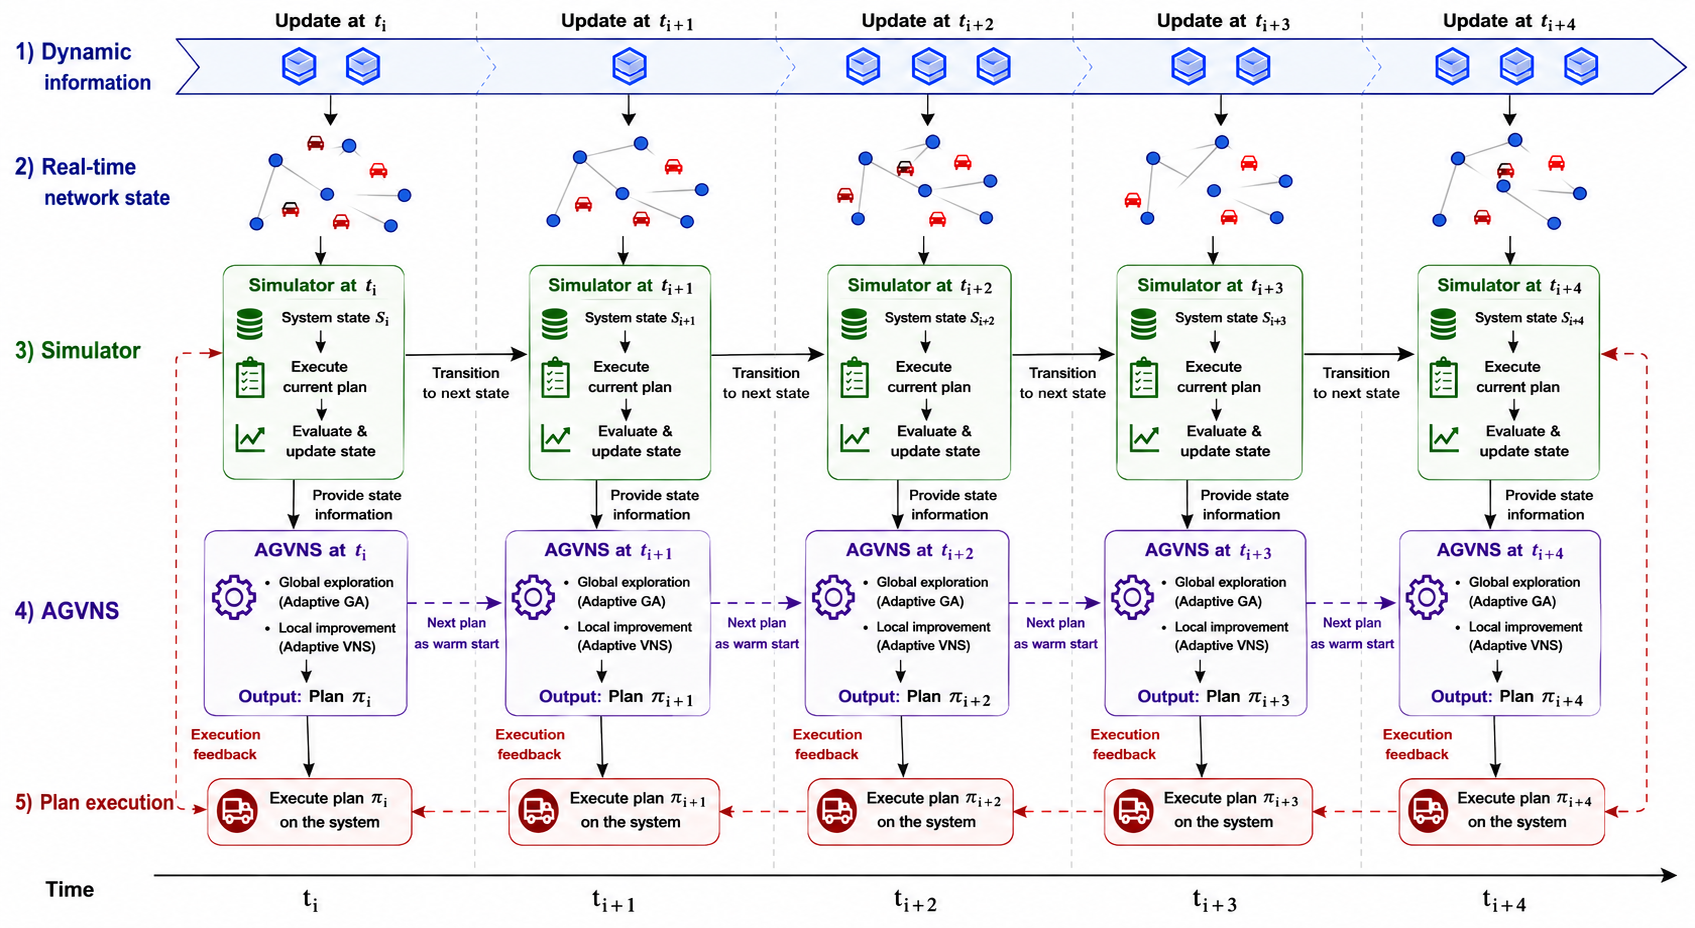
\includegraphics[width=0.85\linewidth]{figure/simulator.png}
%     \caption{Sequential decision process.}
%     \label{fig:sequential_process}
% \end{figure}

% In the sequential decision process illustrated in Figure \ref{fig:sequential_process}, the system evolves through discrete update points $t_i, t_{i+1}, t_{i+2}, \dots$, which occur periodically at intervals of $ \Delta t$ throughout the operation horizon. The initial time is set as $ t_0 = 0$, and the process continues until the final order in the simulation scenario is completed, making the total number of update times finite and dynamically determined by the scenario’s termination. At each update point, new dynamic information, such as customer requests and vehicle states, is collected and integrated into the simulator, which provides an up-to-date snapshot of the system. Based on this information, the \gls{aglisa} algorithm generates a feasible routing plan for the fleet that balances operational objectives. The plan is then executed until the next update point, when new information is again incorporated and a re-optimization is triggered. This iterative cycle of updating, simulation, and optimization allows the system to continuously adapt to dynamic changes in the environment.

% In detail, at the $i$-th update time, the simulator updates collects the newly released orders during the previous time period. Specifically, the set of new orders $O^i_{\text{new}}$, which are released within the time interval $[t_i - \Delta t, t_i]$, is collected. In addition, the simulator retrieves the set of uncompleted orders $O^i_{\text{uncompleted}}$, i.e., the orders released in $[t_0, t_i - \Delta t]$ that have not yet been served. For the re-optimization procedure, we treat these as a unified set

% $$
% O^i = O^i_{\text{new}} \cup O^i_{\text{uncompleted}}.
% $$

% Moreover, the simulator provides up-to-date information on the fleet of vehicles, including:

% \begin{itemize}
%     \item The current locations of vehicles $\theta^i = \{ \theta^i_k \mid k = 1, \dots , K \}$.
%     \item Their destinations $\phi^i = \{ \phi^i_k \mid k = 1, \dots, K \}$, which are determined based on the previous optimization results. Each $\phi^i_k$ also specifies the items to be loaded or unloaded at the next location, i.e., $\phi^i_k = (f^{i , k}_{\text{next}}, c^{i , k}_{\text{next}})$, where $c^k_{\text{next}}$ is the set of order items associated with that stop.
%     \item The currently carried items of each vehicle $\gamma^i =  \{\gamma^i_k \mid k = 1, \dots , K\}$.
% \end{itemize}

% Other essential data, such as the route network $G$, the set of factories $F$, and the set of arcs $A$, are also maintained. Combined, these components provide the complete set of information required for the re-optimization process:

% $$
% (G, F, A, O^i, \theta^i, \phi^i, \gamma^i).
% $$

% After obtaining the updated information, the simulator triggers a re-optimization step, during which a new decision is made by the algorithm. A decision corresponds to a feasible routing plan for the entire fleet of vehicles. Formally, at the $i$-th update point, let $\Omega^i$ denote the set of all possible tuples of feasible and mutually compatible route plans for the vehicles. From this set, exactly one tuple must be selected:

% $$
% R^i = \big( r^{i , k} \mid k = 1, \dots , K \big), \quad R^i \in \Omega^i.
% $$

% Here, each $r^i_k$ represents the route plan assigned to vehicle $k$. Each route must satisfy all problem constraints, along with an additional consistency requirement: if $r^i_k$ is non-empty, then the first factory visited in $r^i_k$ must coincide with the destination of the current plan $\phi^i_k$, and the associated item set at this location must remain consistent. Formally,

% $$
% \phi^i_k = m^{i , k}_1.
% $$

% As a result, the selected tuple $R^i$ defines the feasible set of coordinated route plans that serves as the operational decision at update time $t_i$. These plans are then executed by the vehicles until the next update point, when a new re-optimization is triggered.

\subsection{Framework}

\begin{figure}[h!]
    \centering
    \makebox[\textwidth][c]{%
        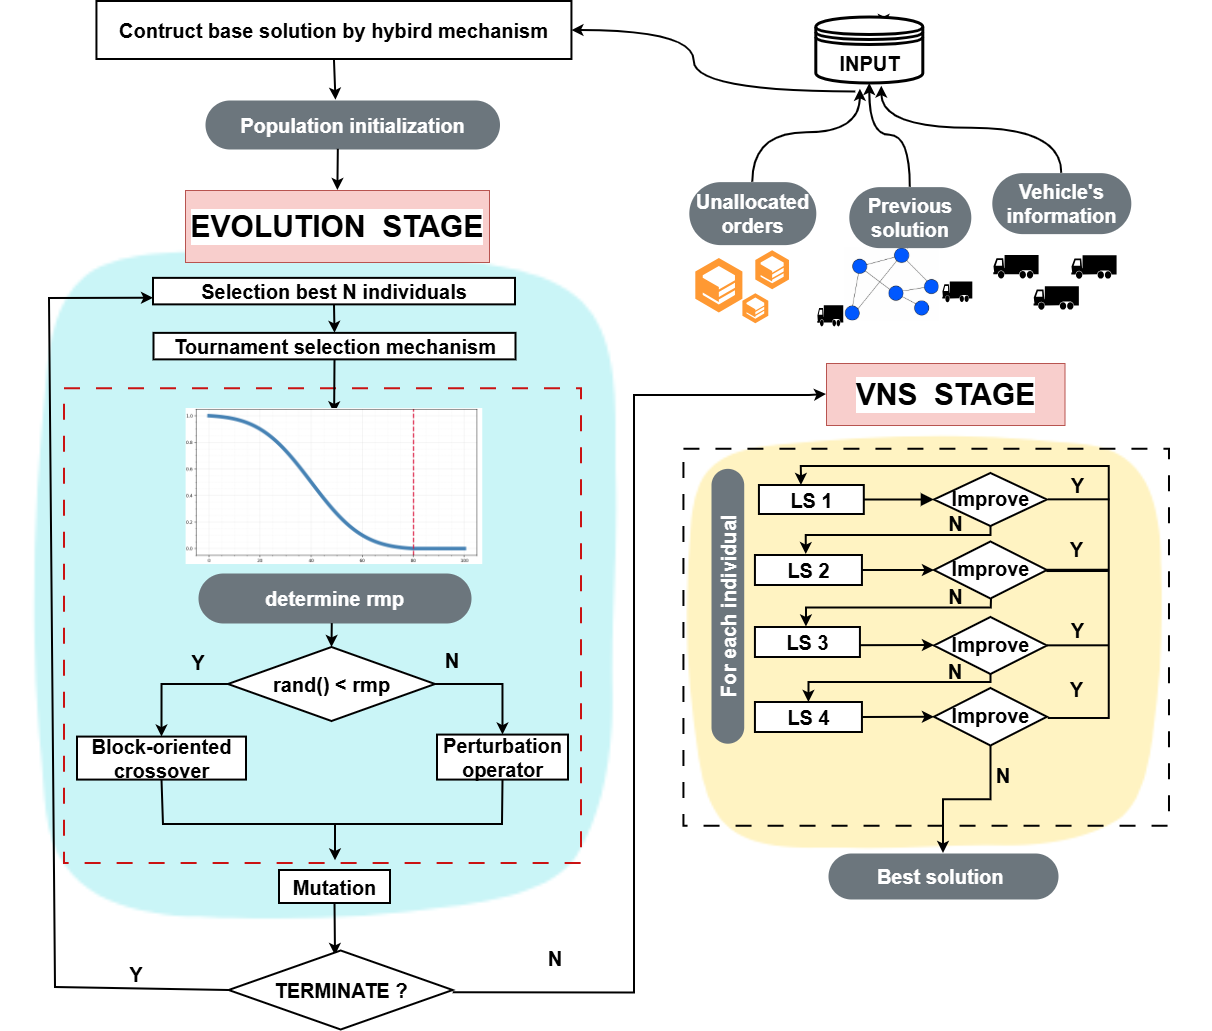
\includegraphics[width=1\linewidth]{figure/frame.png}%
    }
    \caption{General framework}
    \label{fig:main_fig}
\end{figure}

Our proposed approach is divided into two main phases: the Evolution Stage and the \gls{vns} Stage, as illustrated in Figure~\ref{fig:main_fig}. At each re-optimization epoch, the algorithm receives (i) the set of unallocated orders $O_t$ (new and previously unserved requests), (ii) the previous routing solution $R_{t-1}$, and (iii) the current vehicle states $V_t$ (location, committed next node, and on-board load). The previous solution is first cleaned by removing all fully served, yielding a valid partial solution. Next, every new order whose demand exceeds vehicle capacity $Q$ is split into feasible sub-orders that retain the original pickup and delivery locations. The resulting set of requests, together with the partial routes and current vehicle states, is then passed to the hybrid initialization procedure to construct a feasible high-quality seed solution for the new static \gls{pdp} subproblem.

The evolution stage begins by constructing a high quality seed solution \(x^0\) from the warm started partial routes using an advanced hybrid construction heuristic, then generates a diverse initial population of size \(p_{size}\) by repeatedly destroying a random fraction of requests in \(x^0\) and random reconstructing them. A steady state memetic loop is then executed: tournament selection forms the mating pool; for each of the \(p_{size}\) offspring, the adaptive crossover ratio decides whether to apply the block-oriented crossover or a destroy-and-reconstruct perturbation. After all offspring are generated, only the top-ranked subset undergoes adaptive mutation, where one of the four local search operators is selected using roulette-wheel selection based on their historical success rates. Each offspring replaces the worst population member if it is better, preserving elitism. The loop terminates when reaching the generation limit, time budget, or convergence, and the population is passed to the \gls{vns} Stage for final intensification.

Upon completion of the evolution stage, the refined population is transfered to the \gls{vns} stage for local optimization. First, a filter is applied to eliminate duplicates, ensuring population diversity and potential. The stage then applies a hierarchical sequence of local search operators to each surviving solution. These operators are organized in an adaptive decision-tree structure, in which they are sequentially tested for improvement, and the order of application is dynamically adjusted for each individual solution. If an operator yields a better solution, the process restarts from the top of the hierarchy; otherwise, it proceeds to the next. This descent mechanism systematically explores variable neighborhoods until no further improvements are possible, culminating in the identification of the best solution found. This hybrid approach effectively balances global exploration via genetic evolution with intensive local exploitation through \gls{vns}, enhancing solution quality for the static \gls{pdp} subproblems within our periodic re-optimization framework.

\subsection{Evolution stage}
\subsubsection{Solution representation}

A feasible solution to the static \gls{pdp} subproblem is represented as a set of vehicle routes, where each route is an ordered sequence of nodes. For a fleet of homogeneous vehicles, each chromosome encodes the assignment of requests to vehicles and the sequencing within each route. Each request $o^i$ corresponds to a pair of nodes: a pickup node $i^+$ and a delivery node $i^-$, with the precedence constraint enforced such that $i^+$ always precedes $i^-$ in the same route. Vehicle capacity constraints are respected, and time windows (if applicable) are checked during the feasibility evaluation.

Figure~\ref{fig:sol_repre} illustrates an example solution with three vehicles serving nine requests. Routes are color-coded: green for $V_1$ (serving requests 4, 2, 5), blue for $V_2$ (requests 1, 3, 6, 7), and purple for $V_3$ (requests 8, 9). The lower part depicts the explicit node sequences, highlighting the paired pickup-delivery structure. This representation facilitates genetic operations such as crossover and mutation, which preserve feasibility by treating pickup-delivery pairs as atomic blocks where possible, while allowing flexible reassignments across vehicles.

%This representation enables the seamless incorporation of preprocessed partial solutions, treats inherited pickup-delivery pairs as atomic blocks for stability, and supports efficient feasibility-preserving operations - paving the way for the population initialization, adaptive crossover, and mutation mechanisms detailed in the subsequent subsections before transitioning to the Variable Neighborhood Search stage for further refinement.


\begin{figure}
    \centering
    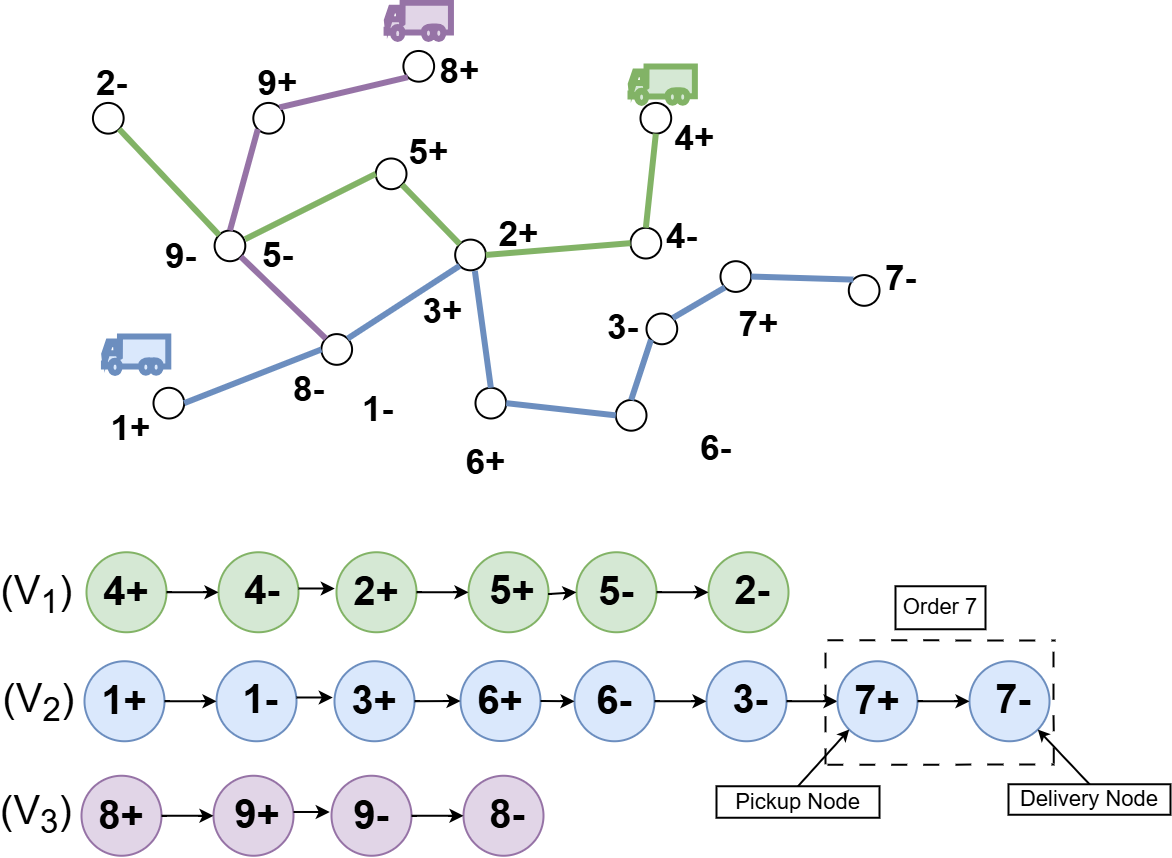
\includegraphics[width=0.8\linewidth]{figure/representation.png}
    \caption{Illustration of the solution representation. Each color denotes a vehicle route, where nodes are labeled by order index and pickup (+) or delivery (–) type. The bottom part presents the corresponding route sequences for vehicles $V_1$, $V_2$ and $V_3$.
    }
    \label{fig:sol_repre}
\end{figure}

\subsubsection{Population initialization}


\begin{algorithm}[ht!]
\caption{Hybrid Greedy Initialization Procedure}
\label{alg:initialization}
\SetAlgoLined
\LinesNumbered
\DontPrintSemicolon
\SetKwInOut{Input}{Input}
\SetKwInOut{Output}{Output}

\Input{
    $O_t^{new}$: set of new customer orders emerged in period $t$ \\
    $\{v^k\}_{k \in K}$: current state and remaining route of each vehicle \\
    $f(\cdot)$: objective function defined in \autoref{eq:f}\\
}
\Output{$x^0$: high-quality feasible initial solution}

$minCost$ $\leftarrow +\infty$\;
$x^0 \leftarrow$ repaired previous partial solution\;

\ForEach{new order $o^i \in O_t$}{
    \ForEach{vehicle $v^k \in K$}{
        $U_k \leftarrow$ set of unfinished nodes currently in the route of $v_k$\;
        
        \eIf{$|U_k| + 2 \leq 8$}{
            Enumerate all feasible combination if $o^i$ is inserted into $v_k$\;
            
            Let $x_{\min}^k$ be the insertion that yields the smallest value\;
            \If{$f(x_{\min}^k) < minCost$}{
                $minCost$ $\leftarrow f(x_{\min}^k)$\;
                Record the updated route of $v_k$ as the best temporary insertion\;
            }
        }{
            Perform cheapest feasible insertion of $o^i$ into $v_k$  \;
        }
    }
    Insert $o^i$ into best-found position \;
    Update solution $x^0$ \;
}
\Return $x^0$\;
\end{algorithm}

Following the solution representation introduced in the previous subsection, the initial population for the evolution stage is carefully constructed to balance solution quality, feasibility, and diversity. This step is designed to generate a high-quality initial population by incorporating effective seeding strategies, thereby accelerating convergence toward superior solutions.

The procedure commences with the generation of a single high-quality base solution $x^0$ using a hybrid  construction heuristic, as outlined in algorithm~\ref{alg:initialization}. This heuristic sequentially assigns each new order $o^i \in O_t^{new}$ to the most suitable vehicle and position within its current partial route. To achieve this, for every vehicle $v^k$, the algorithm first assesses the complexity of the insertion: if the number of unfinished nodes in $v^k$'s route ($|U_k|$) plus the two nodes from $o^i$ is small (e.g., $\leq 8$), all possible feasible permutations for the pickup-delivery pairs are exhaustively enumerated. Feasibility is checked against precedence (pickup before delivery), capacity (no overload at any point), and time windows (if applicable), with the insertion yielding the minimal increase in the objective function $f(\cdot)$ - typically a weighted sum of travel distance, time, and delay penalties as defined in \autoref{eq:f}- being selected. For vehicles with longer routes where enumeration would be computationally prohibitive, a faster cheapest insertion heuristic is employed: the pickup and delivery nodes are inserted at positions that minimize the detour cost, computed via efficient distance lookups or approximations. Across all vehicles, the global best insertion (lowest $minCost$) is chosen for $o^i$, and the solution $x^0$ is updated accordingly. This hybrid approach ensures that $x^0$ is not only feasible but also competitive in quality, serving as an effective seed that inherits the strengths of the repaired previous solution.

% \begin{algorithm}[ht!]
% \caption{Population Initialization}
% \label{alg:population_init}
% \SetAlgoLined
% \LinesNumbered
% \DontPrintSemicolon
% \SetKwInOut{Input}{Input}
% \SetKwInOut{Output}{Output}

% \Input{
%     $x^0$: heuristically generated routes \\
%     $O_t$: Unallocated order in current timestep \\
%     quantity: desired population size
% }
% \Output{population: list of diverse feasible chromosomes}

% population $\leftarrow \emptyset$\;

% \uIf{$O_t$ contains at least 2 orders}{
%     \While{$|$population$| < $quantity}{
%         $x \leftarrow$  randomly break and re-insert 50\% of orders of $x^0$ \;
%         \If{$x$ is feasible}{
%             population.append($x$)\;
%         }
%     }
% }
% population.append($x^0$) \tcp{ensure include warm-start solution}
% \Return population\;
% \end{algorithm}

Once $x^0$ is obtained, the full population of size $quantity$ is generated through controlled diversification. Provided there are at least two orders in $O_t$ to allow meaningful variation, the algorithm iteratively creates new chromosomes by perturbing $x^0$. Specifically, approximately 50\% of the orders in $x^0$ are randomly selected and removed (while maintaining route integrity), then re-inserted using the same cheapest insertion logic as in the heuristic, but with randomized vehicle and position choices to introduce variability. Each perturbed solution $x$ is validated for feasibility; only valid ones are added to the population. To preserve elitism and ensure the best-known starting point is not lost, the original $x^0$ is always appended to the population. This perturbation rate of 50\% strikes a balance: too low would yield overly similar individuals, risking local optima entrapment, while too high might degrade quality excessively. In cases with fewer orders, the population may be smaller or fallback to $x^0$ alone, though this is rare in practical dynamic scenarios.

%Empirically, this initialization strategy has been shown to outperform random or purely constructive methods in PDP variants by reducing the number of generations needed for convergence and improving overall solution robustness. It directly sets the foundation for the adaptive crossover operator (next subsection), where parental solutions from this diverse yet strong population are recombined, and for the mutation operators that locally refine them, ultimately feeding into the Variable Neighborhood Search stage for deeper exploitation.

\subsubsection{Adaptive crossover operator}
\label{sec:adap_cross}
% chỗ này cần trình bày phép lai ghép, động lực tại sao phải sử dụng adaptive crossover ratio
% mã giả crossover và trình bày
% \begin{algorithm}[ht!]
% \caption{Block-Oriented Crossover}
% \label{alg:crossover}
% \SetAlgoLined
% \LinesNumbered
% \DontPrintSemicolon
% \SetKwInOut{Input}{Input}
% \SetKwInOut{Output}{Output}

% \Input{parent1, parent2: parent solutions \\
%        base\_plan: fixed part of routes \\
%        }
% \Output{child: feasible offspring}

% \texttt{block\_pool} $\leftarrow$ Extract contiguous node blocks from both parents \;
% \texttt{used\_order} $\leftarrow$ orders in base\_plan \;
% \texttt{stagnation} $\leftarrow$ 0 \;

% \While{not terminated}{

%     Update \texttt{block\_pool} (salvage overlaps from previous insertion) \;
    
%     Score remaining blocks  \;
    
%     best\_block $\leftarrow$ skyline-dominant block with the most unused orders \;
    
%     Find the cheapest end-of-route insertion \;

%     \eIf{insertion is feasible (Capacity + LIFO)}{
%         Commit block to child \;
%         Update \texttt{used\_order} \;
%         \texttt{stagnation}  $\leftarrow$ 0 \;
%     }{
%         Discard block \; 
%         \texttt{stagnation} ++ \;
%     }
% }

% Remove duplicate nodes from the child solution \;
% Reinsert any missing order into the child \;

% \Return child \;
% \end{algorithm}

A node block (denoted as \textit{NB}) for request \(o^i\) is a contiguous subsequence of a vehicle route that starts at the pickup node \(i^+\) and ends at the delivery node \(i^-\). By definition, it satisfies the precedence constraint \(i^+ \prec i^-\), with all intermediate nodes (which may belong to other requests) served after \(i^+\) and before \(i^-\), while preserving overall route feasibility. By construction, every \textit{NB} automatically respects the LIFO discipline within its scope and typically exhibits locally optimal characteristics in high-performing solutions.

Classical crossover operators for vehicle routing problems frequently violate pickup-delivery precedence or capacity constraints and destroy these high-quality contiguous blocks, leading to infeasible or severely degraded offspring. To overcome these shortcomings, we propose a block-oriented crossover that explicitly extracts well-optimized blocks from both parents and selectively recombines them. By inheriting historically effective sub-routes from previous optimization steps and treating them as strong memetic building blocks, the operator constructs offspring that balance travel distance, service time, and load distribution while maximizing coverage of yet-unassigned requests. This strategy not only ensures feasibility and diversity but also significantly accelerates convergence in the time-constrained dynamic PDP environment, where warm-starting is essential. %The complete procedure is detailed in Algorithm~\ref{alg:crossover}.

The operator initializes with a base solution containing committed route portions that must remain fixed to honor ongoing vehicle states. From both parent chromosomes, contiguous node blocks are systematically extracted, each corresponding to a specific request. These blocks are aggregated into a unified block pool. 

Each block \textit{NB} with edge set \(E\) and item set \(I\) in the pool is then evaluated using a multi-objective scoring function that computes normalized averages for key metrics: average travel distance (\(\bar{d}\)) as the mean edge length, average service time (\(\bar{t}\)) reflecting traversal duration, and average load (\(\bar{q}\)) capturing demand distribution across items.

\begin{equation}
\bar{d} = \frac{\sum_{(u,v) \in E} d_{uv}}{|E|}.
\end{equation}
\begin{equation}
 \quad \bar{t} = \frac{\sum_{(u,v) \in E} t_{uv}}{|E|}.
\end{equation}
\begin{equation}
 \quad \bar{q} = \frac{\sum_{i \in I} \text{demand}(i)}{|I|}.
\end{equation}

To handle the multi-objective nature efficiently, a skyline (Pareto) filter is applied to retain only non-dominated blocks, those not outperformed in all metrics by any other. Among these, prioritization favors blocks that introduce the maximum number of unassigned requests (i.e., requests not yet assigned in the child or covered by the fixed scaffold).

The recombination operator constructs the offspring iteratively in a greedy fashion. At each iteration, the highest-priority block is selected and appended to the most suitable vehicle route using an append-only cheapest-insertion heuristic that minimizes additional detour cost while maintaining incremental feasibility. Upon successful insertion, the block is permanently fixed, its requests are marked as covered, and any remaining blocks that overlap with it are salvaged: overlapping portions are discarded, and each resulting non-empty contiguous residual segment is converted into a new feasible block before being reinserted into the priority pool. This salvage mechanism promotes block reuse and improves overall solution coverage.

In cases of insertion failure or insufficient request gain (below a predefined threshold for unassigned requests), the block is permanently discarded from the pool, and a stagnation counter is incremented to detect unproductive loops. The iteration terminates upon reaching full request coverage (all required PDP requests assigned), a global timeout aligned with the re-optimization epoch budget, maximum iterations, or excessive stagnation.

Following the main loop, a comprehensive repair phase ensures solution integrity: redundant orders are pruned to eliminate inefficiencies, and any missing requests are individually reinserted using a standard cheapest-insertion heuristic applied across vehicles. This guarantees that the offspring is both complete (serving all unallocated requests) and feasible, ready for further refinement.

% động lực cho adaptive crossover ratio
In large-scale Dynamic Pickup-and-Delivery Problems, the computational budget available for each re-optimization epoch is extremely tight typically 10 minutes, the size of the static subproblem \(N_t\) (number of currently unallocated requests) fluctuates dramatically over time. During off-peak periods, \(N_t\) may be as low as 5–20 requests; during rush hours, it can easily exceed 200–400 requests.

Empirical observation on real-world and benchmark instances consistently reveals the following pattern.
In small instances: Block-oriented crossover yields significant improvements due to manageable search space and effective recombination of high-quality parental blocks. In large instances, the crossover benefit diminishes sharply; most gains come from fast local operators (mutation and VNS), as crossover becomes costly and produces offspring that are quickly outperformed by local search.

Using a fixed crossover ratio (e.g., the conventional 0.8–1.0) therefore wastes precious time on large instances and under-exploits the global search potential on small ones. This inefficiency is particularly costly in dynamic settings, where every millisecond saved in one epoch directly translates into better solutions in subsequent epochs.

To allocate the scarce computational resource optimally, we introduce an adaptive crossover probability that automatically scales with the current problem size. When few requests are present, the algorithm aggressively performs block recombination for broad exploration; as the number of requests grows, the crossover probability decays smoothly, gracefully shifting the budget toward the more rewarding mutation and Variable Neighborhood Search stages. This simple yet effective adaptation ensures that the expensive block-oriented crossover is applied exactly where it matters most, providing a natural, parameter-light mechanism to maintain high solution quality across the entire spectrum of dynamic workload conditions. The adaptation is based on the complementary error function (ERFC), which provides an infinitely differentiable, monotonic, sigmoid-like transition with minimal parameterization.

% Trình bày về adaptive crossover
\begin{figure}
    \centering
    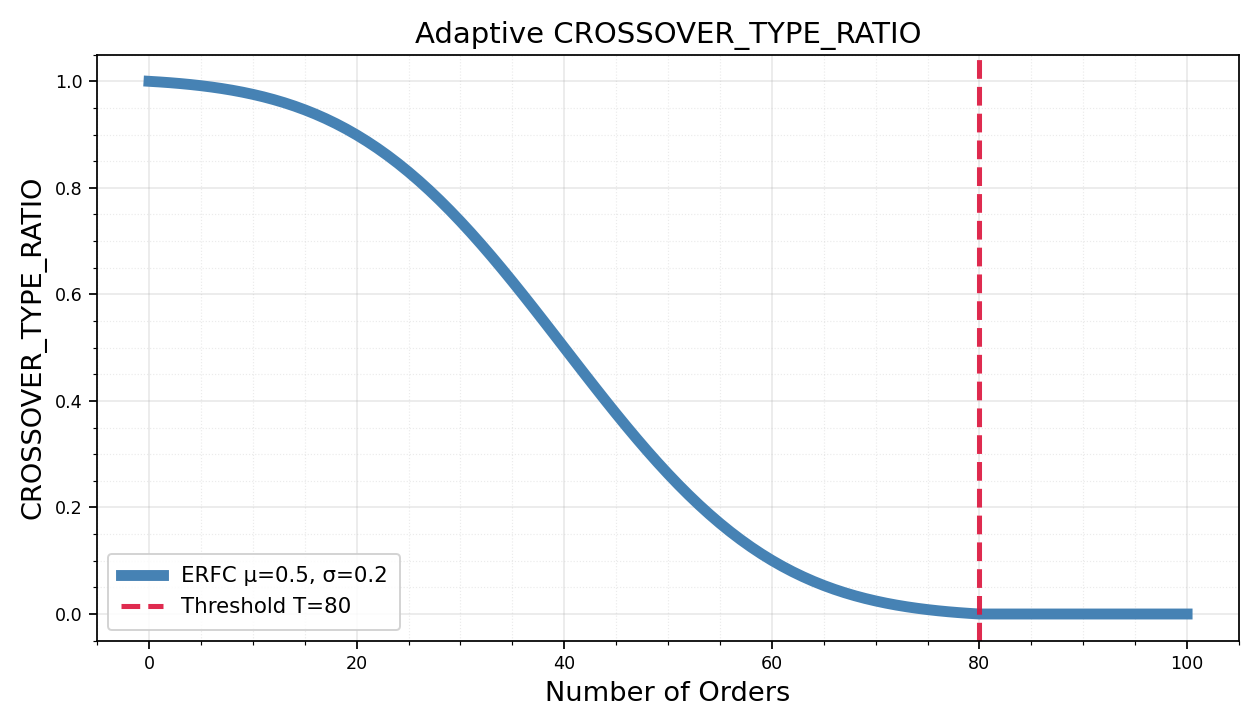
\includegraphics[width=1\linewidth]{figure/ERFC.png}
    \caption{The Applied $\text{ERFC}$ function. The graph illustrates the distribution used in the model, characterized by parameters $\mu = 0.5$, $\sigma = 0.2$ and $T = 80$.
    }
    \label{fig:ERFC}
\end{figure}

Formally, let \(T > 0\) be a reference problem-size threshold (the quantity of unallocated orders) and define the normalized load factor  

\begin{equation}
p = \min\!\left(1,\frac{n}{T}\right).
\end{equation}

The raw decay function is  

\begin{equation}
g(p) = \frac{1}{2}\operatorname{erfc}\!\left(\frac{p-\mu}{\sigma\sqrt{2}}\right),
\end{equation}

where \(\mu \in [0,1]\) is the inflection point and \(\sigma > 0\) controls the steepness. The boundary values are  

\begin{equation}
g(0) = \frac{1}{2}\operatorname{erfc}\!\left(\frac{-\mu}{\sigma\sqrt{2}}\right),\qquad 
g(1) = \frac{1}{2}\operatorname{erfc}\!\left(\frac{1-\mu}{\sigma\sqrt{2}}\right).
\end{equation}

Normalization to the unit interval yields  

\begin{equation}
w(p) = \frac{g(p)-g(1)}{g(0)-g(1)},
\end{equation}

which satisfies \(w(0)=1\) and \(w(1)=0\) exactly. The adaptive crossover probability is then defined as  

\begin{equation}  
\text{ratio}(n)=\begin{cases}
w\!\left(\min\!\left(1,\frac{n}{T}\right)\right) & \text{if }n < T,\\[4pt]
0 & \text{if }n \ge T\}.
\end{cases}  
\end{equation}

The resulting function is \(C^\infty\)-smooth and requires only three intuitive parameters: \(\mu\) determines where the decay begins, while \(\sigma\) adjusts its rapidity and $T$ control the convergent value. Consequently, the block-oriented crossover is applied intensively on small instances, gradually phased out as the instance grows, and (if the hard cutoff is enabled) completely disabled beyond \(T\), thereby redirecting all remaining time to mutation and variable neighborhood search. This simple yet mathematically elegant mechanism automatically balances global exploration and local exploitation across the full spectrum of dynamic workloads without requiring online learning or complex scheduling heuristics. In  \autoref{fig:ERFC}, we illustrate a specific use case of our proposed distribution. 

\subsubsection{Mutation operators}

\begin{figure}
    \centering
    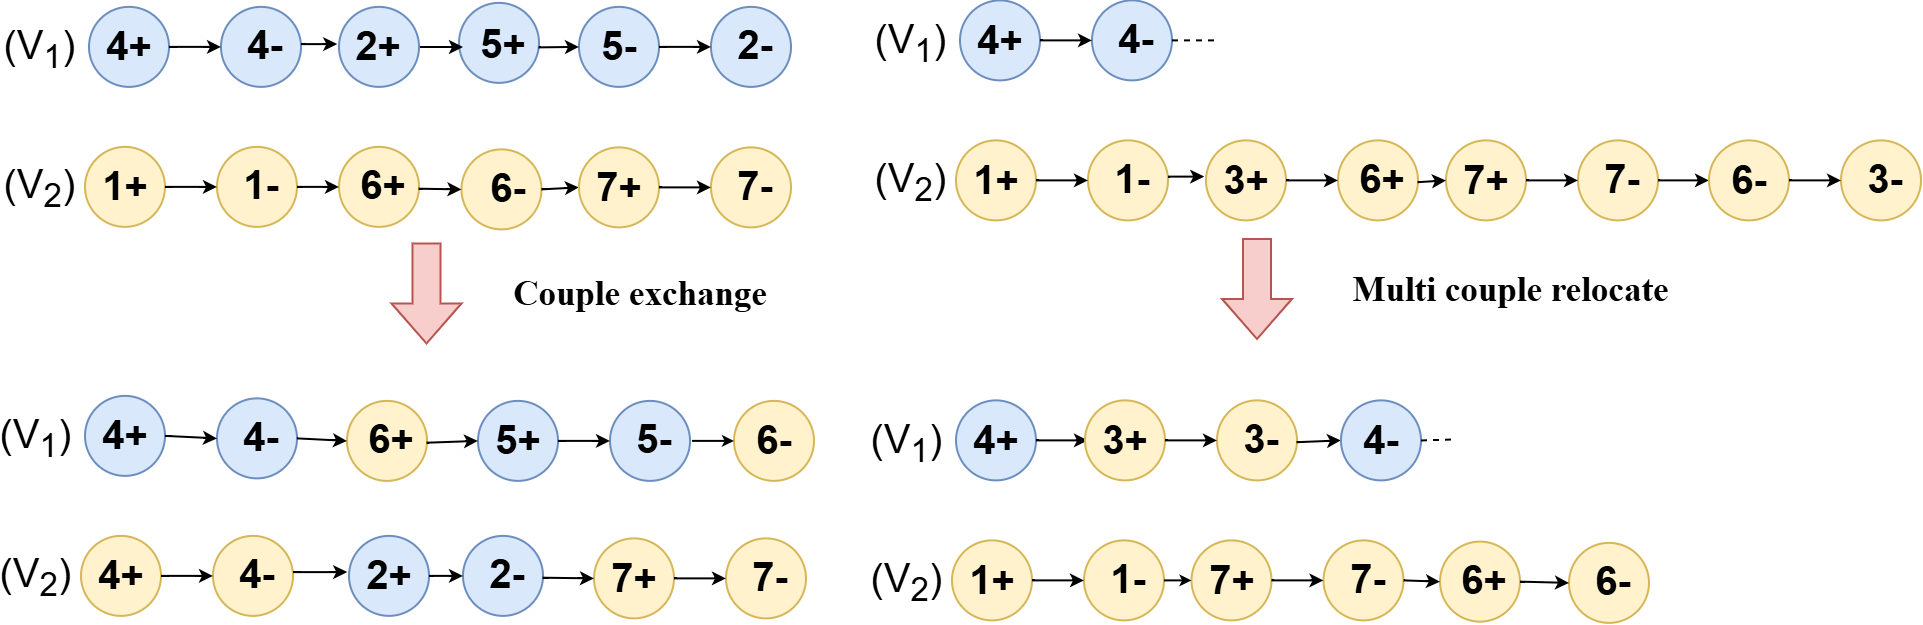
\includegraphics[width=1\linewidth]{figure/Couple_LS.png}
    \caption{The illustration of Couple exchange and Multi couple relocate}
    \label{fig:couple_LS}
\end{figure}

\begin{figure}
    \centering
    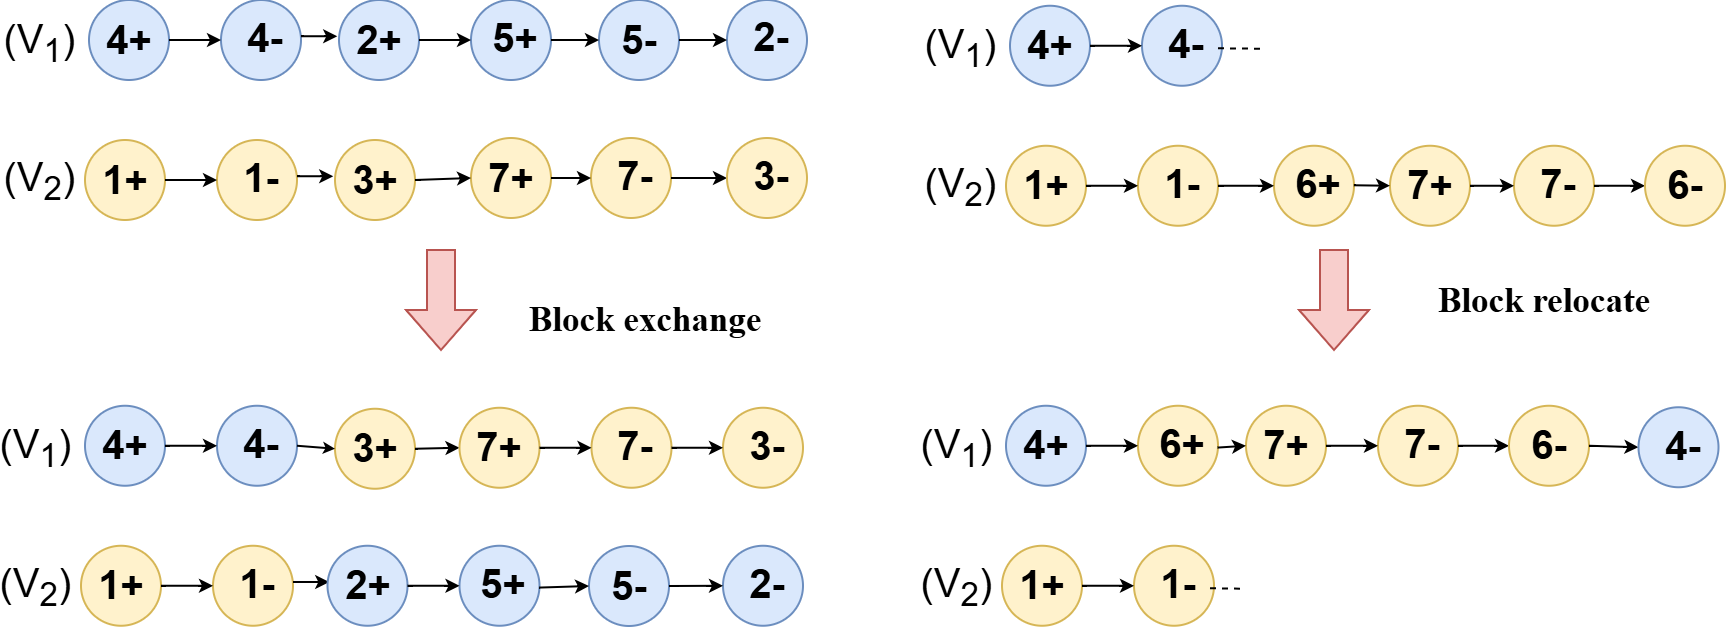
\includegraphics[width=1\linewidth]{figure/Block_LS.png}
    \caption{The illustration of Block exchange and Block relocate}
    \label{fig:block_LS}
\end{figure}

The mutation phase employs four hierarchical, request-centric neighborhood operators specifically tailored for the pickup-and-delivery structure. Each operator treats a complete request (i.e., its full pickup-delivery sequence) as an indivisible unit, thereby preserving precedence and LIFO constraints by construction. The operators are illustrated in Figures~\ref{fig:couple_LS} and~\ref{fig:block_LS}.

\begin{itemize}
    \item \textbf{Couple-Exchange}  
    Exhaustively evaluates all pairs of distinct requests in the current solution (regardless of vehicle assignment) and identifies the single best swap of their entire pickup-delivery sequences — simultaneously exchanging the pickup node(s) of one request with those of the other and the corresponding delivery node(s) (Figure~\ref{fig:couple_LS}, left). This deterministic best-swap strategy delivers highly effective load rebalancing and request reassignment in $O(n^2)$ time, where $m$ is the number of active requests.

    \item \textbf{Multi-Couple Relocate }  
    Performs a complete scan of the solution to detect every request whose relocation to any feasible position (same or different vehicle) would reduce the objective. All improving relocations are inserted into a priority queue ordered by expected gain. The best candidate is executed, the solution is updated, and the process repeats until no further improving move remains in the queue (Figure~\ref{fig:couple_LS}, right).

    \item \textbf{Block-Exchange }  
    Considers contiguous route segments (blocks) of arbitrary length, each starting with a pickup node and ending with the matching delivery node of the last request in the sequence. The operator enumerates all pairs of blocks and swaps them entirely (Figure~\ref{fig:block_LS}, left). This large-scale restructuring preserves high-quality internal sub-sequences while enabling dramatic reconfiguration of the solution.

    \item \textbf{Block-Relocate}  
    For each contiguous block, evaluates all feasible insertion positions (including within its original route) and relocates the block to the position offering the greatest cost reduction (Figure~\ref{fig:block_LS}, right). As the most disruptive neighborhood, it serves as an effective shaking mechanism when finer-grained operators stagnate.
\end{itemize}

All four operators rely on incremental feasibility checks (capacity stack + LIFO simulation) and exhibit $O(m^2)$ (or $O(m^3)$ for LS2) worst-case complexity, where $m$ is the number of active requests. In high-dynamism epochs with $m \ge 400–500$, exhaustive exploration can exceed the strict per-epoch time budget.

To preserve scalability, the same threshold $T$ defined for the adaptive crossover ratio (Section~\ref{sec:adap_cross}) is reused as a trigger for a fast request aggregation  procedure. Whenever $m \ge T$, requests that share identical pickup and delivery locations and appear consecutively (or nearly consecutively) in at least one current route are temporarily merged into a single super-request. The merged entity is treated as an indivisible unit during the subsequent local-search phase, significantly reducing the effective number of search entities while preserving the precedence and LIFO constraints exactly. Aggregation is completely reversed before the final solution is returned. This mechanism ensures that local-search operators remain computationally viable across the full spectrum of dynamic workloads encountered in large-scale real-world scenarios.

% Mã giả
% \begin{algorithm}[ht!]
% \caption{Mutation Operator}
% \label{alg:mutation}
% \SetAlgoLined
% \LinesNumbered
% \DontPrintSemicolon
% \SetKwInOut{Input}{Input}
% \SetKwInOut{Output}{Output}

% \Input{$x$: chromosome \\
%        \texttt{x.score}: operator success counters \\
%        $f(\cdot)$: objective function}

% $\mathit{op} \leftarrow$ RouletteWheelSelect(\texttt{x.score}) \;
% $x' \leftarrow \mathit{op}(x)$  \tcp[r]{Budget: \textbf{LS\_MAX\_TIME\_PER\_OP}}
% \If{$f(x') < f(x)$}{
%     $x \leftarrow x'$ \;
%     \texttt{x.score[op]} $\leftarrow$ \texttt{x.score[op]} $+ 1$ \;
% }
% \end{algorithm}

After each generation, the $p_{size}$ newly created offspring are merged with the current population, and the best $N$ individuals are retained (elitist steady-state replacement). Mutation is then applied selectively to only the top-$k$ ranked solutions in this updated population (typically $k \approx N/2$).

Mutation operator is applied selectively to only the top-$k$ individuals of the updated population after elitist steady-state replacement. Each selected chromosome maintains a private success-history vector for the four operators; the next operator is chosen via roulette-wheel selection biased toward those that have historically yielded improvements for that lineage, and is executed exhaustively within a strict per-operator time budget, with its counter incremented upon success. This focused, self-adaptive mechanism concentrates intensive local improvement on the current elite set while automatically learning the most effective neighborhoods for each high-quality solution lineage — knowledge that is directly reused in the subsequent VNS stage to initialise the search order with the historically best-performing operators, thereby significantly accelerating final convergence without introducing any additional parameters.

\subsection{Variable neighborhood search stage}
The second component of our algorithm is the \gls{vns} stage, which is incorporated to further enhance the solution quality obtained from the evolutionary stage. Acting as an intensification mechanism, VNS systematically explores multiple neighborhood structures to escape local optima and refine routing plans. At the start of this stage, a set of unique, high-quality solutions is selected from the final evolved population to serve as distinct starting points for VNS; duplicates  are filtered out so that the search is applied to diverse promising regions of the solution space.

The VNS framework iteratively applies a set of neighborhood operators, as illustrated in \autoref{fig:block_LS} and \autoref{fig:couple_LS}. For each neighborhood, a corresponding local search procedure is executed to perform fine-grained exploitation within that structure. When an improved solution is found, it replaces the current one and the search restarts from the first neighborhood; if no improvement is achieved, the procedure advances to the next neighborhood in the predefined sequence.

The ordering of local search operators is dynamically adapted based on their self-improvement history during the evolutionary stage—operators that have produced more successful improvements are given higher priority. The VNS search for each selected individual terminates once none of the four operators can produce further improvements consecutively.

By selecting distinct top-performing solutions and applying this intensive VNS refinement to each, the hybrid strategy balances focused exploitation with population-level diversity. This combination increases the likelihood of discovering high-quality solutions across different promising regions of the search space, which is particularly important for large-scale and time-constrained dynamic scenarios.


\section{Experiments}\label{sec:exp}
\subsection{Experimental settings}
This section details the simulation environment and parameter configurations adopted in our experiments. All simulations and algorithm evaluations were executed on a system equipped with an Intel \textsuperscript{\textregistered} Core\textsuperscript{\texttrademark} i7 processor and 16 GB of RAM. Section \ref{ss:exp-data} introduces the benchmark dataset and its generation procedure. Lastly, Section \ref{ss:exp-params} summarizes the parameter settings applied throughout the experiments.

\subsubsection{Dataset and simulator} \label{ss:exp-data}

%Publicly available datasets for the Dynamic Pickup and Delivery Problem (DPDP) remain limited, as most existing instances are synthetically generated and do not adequately reflect the complexity and uncertainty of real-world operations. Artificial benchmarks, such as the one introduced in , focus mainly on testing algorithmic responsiveness under controlled degrees of dynamism and urgency. In that benchmark, problem instances were generated to represent eight dynamism levels (from 20\% to 100\%) and five urgency settings (ranging from 5 to 45 minutes), forming a total of 200 synthetic scenarios. Other studies typically rely on static Pickup and Delivery Problem (PDP) datasets  or use random instance generators [7,47,59,60,115] to simulate dynamic environments in a simplified way. Although these datasets are useful for algorithmic prototyping, they remain limited in realism and do not reflect real-world dispatching constraints.

 Huawei Technologies released a set of Dynamic Pickup and Delivery Problem benchmarks during the ICAPS 2021 competition \cite{hao2022introduction}. Commonly known as the HW benchmark, this dataset is constructed from thirty days of actual industrial logistics data and therefore represents one of the first large-scale, real-world DPDP testbeds. It integrates several key operational factors—such as vehicle capacity, service time windows, dock availability, and the Last-In-First-Out (LIFO) constraint on loading and unloading—that are typically absent from synthetic datasets.

The HW benchmark includes 64 instances derived from combinations of vehicle and order quantities. Four fleet sizes are considered (5, 20, 50, and 100 vehicles), and eight order volumes (50 to 4000 orders) are used to represent different workload levels. For each configuration, eight daily instances were sampled, resulting in a diverse collection that spans small to large operational scales. Each instance corresponds to a real working day, where customer requests appear gradually over time, reflecting dynamic order arrivals in practice. The dataset’s generation process samples orders and vehicle data from historical records to maintain realistic spatial and temporal distributions.

For analytical convenience, instances are often grouped into three size categories—small, medium, and large—based on the number of requests. Smaller cases contain relatively sparse order arrivals, whereas large-scale cases show frequent and dense request inflows across the working day. This diversity makes the HW benchmark particularly valuable for testing how algorithms perform under varying levels of real-time complexity. Details of the dataset are provided in \autoref{tab:dataset_settings}.

\begin{table}[htbp]
\centering
\caption{Dataset.}
\resizebox{0.7\textwidth}{!}{ 
\begin{tabular}{lccc}
\hline
\textbf{Instance set}  & \textbf{Number of vehicles} & \textbf{Number of orders} \\ 
\hline
Set 1 & 5 & 50 \\
Set 2  & 5 & 100 \\
Set 3 & 20 & 300 \\
Set 4  & 20 & 500 \\
Set 5  & 50 & 1000 \\
Set 6  & 50 & 2000 \\
Set 7  & 100 & 3000 \\
Set 8  & 100 & 4000 \\
\hline
\end{tabular}}
\label{tab:dataset_settings}
\end{table}



The benchmark simulator \footnote{\hyperlink{https://github.com/huawei-noah/xingtian/tree/master/simulator/
dpdp_competition}{https://github.com/huawei-noah/xingtian/tree/master/simulator/
dpdp\_competition}} is initialized using the factory and route information files along with the specified problem instance, after which the simulation process begins. During execution, the simulator invokes the routing algorithm every 10 minutes of simulated time, providing the current system state as input. The algorithm then responds with updated vehicle routes, which are applied to continue the simulation. This iterative interaction continues until all orders have been successfully delivered. Upon completion, the simulator computes the final performance score, defined as a weighted sum of the total travel distance of all vehicles and the cumulative tardiness of customer orders. 

\subsubsection{Parameters setting} \label{ss:exp-params}

All experiments were conducted using a single, fixed parameter configuration for \gls{aglisa} across the entire benchmark of 64 instances. No instance-specific tuning was performed. The complete set of parameters is presented in Table~\ref{tab:parameters}.

\begin{table}[htbp]
\centering
\caption{Parameter configuration of AGVNS}
\label{tab:parameters}
\begin{tabular}{l l}
\toprule
\textbf{Parameter} & \textbf{Value} \\
\midrule
\multicolumn{2}{l}{\textit{Genetic algorithm parameters}} \\
Population size & 40 \\
Max.\ generations per epoch & 20 \\
Parent selection & Tournament selection (size = 8) \\
Replacement strategy & Elitist steady-state \\
Individuals mutated per epoch & Top 25\% \\
Crossover probability & Adaptive (erfc-based, $T{=}80$, $\mu{=}0.5$, $\sigma{=}0.2$) \\
Mutation time budget & 1.0 s \\
\midrule
\multicolumn{2}{l}{\textit{Destroy \& repair operators}} \\
Perturbation strength & Remove 50\% of requests \\
Repair heuristic & Randomised insertion \\
\bottomrule
\end{tabular}
\end{table}

The parameters in Table~\ref{tab:parameters} were applied uniformly to all 64 benchmark instances. This configuration was chosen to provide a balanced trade-off between exploration and exploitation with modest computational effort. The combination of tournament selection, elitist steady-state replacement, and an erfc-based adaptive crossover probability enables \gls{aglisa} to progressively intensify the search while maintaining diversity. The destroy–and–repair mechanism, which removes 50\% of requests and reinserts them using a randomized heuristic, introduces controlled perturbations that help the algorithm escape local optima. No instance-specific tuning was performed to ensure fairness and reproducibility across all experiments.


% AGLISA is benchmarked against the three medal-winning entries from the ICAPS 2021 Dynamic Pickup and Delivery Problem Competition and two additional evolutionary baselines. All algorithms are evaluated in the official unified simulator under identical time limits and hardware conditions.

% - Gold medallist – VNSME \cite{cai2022variable}: Constructs an initial feasible solution through a hybrid heuristic and iteratively improves it using four local-search strategies combined with an efficient disturbance (shaking) mechanism. To date, it remains the published state-of-the-art on the benchmark.

% - Silver medallist: Transforms the dynamic PDP into a series of knapsack-like problems and selectively packs orders into existing routes whenever predefined acceptance thresholds are satisfied.

% - Bronze medallist: Generates an initial solution via cheapest insertion and repeatedly applies a ruin-and-reconstruct strategy with multiple removal and re-insertion operators.

% - MA \cite{zhou2024memetic}: A recent memetic algorithm explicitly designed for real-world dynamic PDP applications. Although the original paper reports results superior to the three ICAPS winners, we faithfully re-implemented its core framework (as discussed in Section \ref{sec:other_algo}) and tested it in the official simulator to guarantee fully comparable conditions.

% - GA baseline: A standard genetic algorithm that mirrors the overall evolutionary phase of AGLISA but employs purely random initialisation (no warm-start or advanced seeding) and fixed crossover and mutation probabilities (0.8 and 0.2, respectively). This baseline isolates the contribution of our proposed innovations.

% All competing methods use their original or officially recommended parameter settings without further modification. The use of the unified benchmark environment eliminates any discrepancies arising from simulator implementation or timing measurement.

\subsection{Experimental results}
\subsubsection{Metrics}
To quantify the performance gain of our proposed algorithm over a baseline method, we report the percentage improvement (\%imp). Let $A$ denote the average objective value obtained by a baseline algorithm and $F$ the average value obtained by the full version of our algorithm. Since the DPDP is a minimization problem, a lower objective value indicates a better solution. The improvement is computed as follows:
\[
\text{\%imp} = \frac{A - F}{A} \times 100\%.
\]

A positive value of \%imp indicates that the full algorithm achieves a lower objective value than the baseline, demonstrating superior performance. A higher \%imp corresponds to a larger performance gain, whereas a negative value implies that the baseline performs better on that instance. This metric provides a consistent way to evaluate the relative benefit of each algorithmic component.

\subsubsection{Ablation study}
To assess the contribution of each major component of the proposed algorithm, we conducted an ablation study by evaluating three variants: (i) Without Evolutionary Stage, which disables the evolutionary search component; (ii) Without the Adaptive Mechanism, which retains the evolutionary operators but removes the adaptive parameter control; and (iii) Full Algorithm (\gls{aglisa}), which includes all proposed components. The comparison was performed on all eight benchmark sets of the competition datasets.

Across all datasets, the full algorithm achieves the best average performance, demonstrating the necessity of integrating both evolutionary stage and adaptive mechanism. Removing the evolutionary stage generally leads to substantial performance degradation, especially on larger and more complex instances (Sets 2, 4, 6, 7, and 8), where the average cost increases by 23\%–93\%. Interestingly, for smaller datasets such as Sets 1 and 3, the lack of the evolutionary search leads to only minor degradation, and even slight improvement in Set 1. This reflects that small and stable instances do not require aggressive exploration, and local refinement alone can sometimes suffice. However, for real-world large-scale dynamic scenarios, the evolutionary operators are clearly essential.

Removing the adaptive mechanism also results in considerable performance drops on most datasets, particularly on Sets 2, 4, 6, 7, and 8, where the gaps range from 15\% to over 90\%. This confirms that adaptive parameter tuning helps the algorithm adjust its search intensity according to the characteristics of each re-optimization period, which is crucial for handling large-scale dynamic scenarios. We also observe mild effects on Sets 1, 3, and 5. These smaller or less dynamic instances do not benefit as strongly from adaptive adjustments, likely because their solution structure is relatively stable across time intervals.

Overall, the results in \autoref{tab:ablation} clearly demonstrate that both components are essential, but their contributions differ depending on problem scale. The evolutionary stage provides the primary improvement for large and difficult instances, while the adaptive mechanism enhances robustness and consistency across dynamic settings. These findings validate the design choices of our algorithm and highlight the complementary roles of the two components.

% \begin{table}[t]
% \caption{Performance comparison of the full algorithm and its ablated variants on eight DPDP instance sets, where the \textit{imp} (\%) measures how much better the full algorithm performs compared to each ablated version.}
% \resizebox{\textwidth}{!}{
% \begin{tabular}{|l|rr|rr|r|}
% \label{tab:ablation}
% \hline
% & \multicolumn{2}{c|}{Without Evolutionary stage} 
% & \multicolumn{2}{c|}{Without the adaptive mechanism} 
% & \multicolumn{1}{c|}{\gls{aglisa}} 
% \\ \cline{2-6}
% \textbf{Dataset}
% & \textbf{Avg} & \textbf{\textit{imp}(\%)} 
% & \textbf{Avg} & \textbf{\textit{imp}(\%)} 
% & \textbf{Avg} 
% \\ \hline

% \textbf{Set 1} & \textbf{1233.01} & -1.21 & 1252.73 & 0.38 & 1247.96 \\ \hline
% \textbf{Set 2} & 33158.62 & 36.44 & 28853.43 & 26.96 & \textbf{21075.27} \\ \hline
% \textbf{Set 3} & 710.99 & 1.03 & \textbf{702.02} & -0.24 & 703.68 \\ \hline
% \textbf{Set 4} & 8818.96 & 30.78 & 8590.96 & 28.94 & \textbf{6104.37} \\ \hline
% \textbf{Set 5} & 11261.29 & 7.14 & \textbf{10410.31} & -0.45 & 10457.00 \\ \hline
% \textbf{Set 6} & 593404.32 & 92.94 & 1580895.24 & 97.35 & \textbf{41878.02} \\ \hline
% \textbf{Set 7} & 3498085.71 & 67.25 & 17962094.50 & 93.62 & \textbf{1145531.17} \\ \hline
% \textbf{Set 8} & 20602700.75 & 23.30 & 29453523.91 & 46.35 & \textbf{15802160.72} \\ \hline

% \end{tabular}
% }
% \end{table}

\begin{table}[t]
\centering
\caption{Performance comparison of the full algorithm and its ablated variants on eight DPDP instance sets, where the \textit{imp} (\%) measures how much better the full algorithm performs compared to each ablated version.}
\label{tab:ablation}
\resizebox{\textwidth}{!}{
\begin{tabular}{|l|rr|rr|r|}
\hline
& \multicolumn{2}{c|}{\textbf{Without Evolutionary stage}} & \multicolumn{2}{c|}{\textbf{Without the adaptive mechanism}} & \multicolumn{1}{c|}{\textbf{AGVNS}} \\ \cline{2-6} 
\textbf{Dataset} & \multicolumn{1}{r}{\textbf{Avg}} & \textbf{imp (\%)} & \multicolumn{1}{r}{\textbf{Avg}} & \textbf{imp (\%)} & \multicolumn{1}{c|}{\textbf{Avg}} \\ \hline \hline
Set 1 & \textbf{1,233.01} & -1.21 & 1,252.73 & 0.38 & 1,247.96 \\ \hline
Set 2 & 33,158.62 & 36.44 & 28,853.43 & 26.96 & \textbf{21,075.27} \\ \hline
Set 3 & 710.99 & 1.03 & \textbf{702.02} & -0.24 & 703.68 \\ \hline
Set 4 & 8,818.96 & 30.78 & 8,590.96 & 28.94 & \textbf{6,104.37} \\ \hline
Set 5 & 11,261.29 & 7.14 & \textbf{10,410.31} & -0.45 & 10,457.00 \\ \hline
Set 6 & 593,404.32 & 92.94 & 1,580,895.24 & 97.35 & \textbf{41,878.02} \\ \hline
Set 7 & 3,498,085.71 & 67.25 & 17,962,094.50 & 93.62 & \textbf{1,145,531.17} \\ \hline
Set 8 & 20,602,700.75 & 23.30 & 29,453,523.91 & 46.35 & \textbf{15,802,160.72} \\ \hline
\end{tabular}
}
\end{table}

\subsubsection{Compare with the existing methods} 

We compare the proposed method against the three top-ranking algorithms from the ICAPS 2021 DPDP competition (Gold - VNSME \cite{cai2022variable}, Silver - IM, Bronze - LS), an adapted implementation of the \gls{ma} in \cite{zhou2024memetic}, \gls{ls} \textcolor{red}{them tai lieu tham khao} and a \gls{ga} baseline. Evaluation criteria include objective value and computational time across 64 benchmark instances.


\autoref{tab:summary} summarizes the frequency with which our proposed algorithm, \gls{aglisa}, outperforms the baseline methods across each set of eight test instances. Overall, \gls{aglisa} demonstrates superior performance across the majority of the datasets. Notably, the algorithm achieves complete dominance (8/8 instances) over the Gold, Silver, and Bronze solvers in several sets (Sets 2–4). In comparison to the established evolutionary baselines, the MA, GA, and our method exhibit highly competitive behavior, outperforming them on nearly all instances across all sets. Even within the more challenging Sets 7 and 8 - where the Gold, Silver, and Bronze solvers occasionally yield superior results - \gls{aglisa} still maintains absolute superiority over both MA and GA. These results collectively indicate that our proposed method provides high - quality solutions across diverse instance groups and effectively competes with both state-of-the-art competition winners and established meta-heuristic approaches.

\begin{table}[htp]
\centering
\caption{Comparison of performance across eight instance sets. Each value indicates how many instances (out of 8) in which \gls{aglisa} algorithm achieves better results than the corresponding baseline method.}\label{tab:summary}
\resizebox{0.5\textwidth}{!}{ 
\begin{tabular}{|l|c|c|c|c|c|c|}
\hline
\textbf{Set}   & \textbf{Gold} & \textbf{Sliver} & \textbf{Bronze} & \textbf{MA} & \textbf{GA} & \textbf{TS}\\ \hline
\textbf{Set 1} & 5             & 8               & 6               & 6           & 8         & 7  \\ \hline
\textbf{Set 2} & 7             & 8               & 8               & 8           & 8         & 8  \\ \hline
\textbf{Set 3} & 8             & 8               & 8               & 6           & 7         & 8  \\ \hline
\textbf{Set 4} & 8             & 8               & 8               & 7           & 8         & 8  \\ \hline
\textbf{Set 5} & 6             & 7               & 8               & 8           & 8         & 8  \\ \hline
\textbf{Set 6} & 6             & 8               & 8               & 8           & 8         & 8  \\ \hline
\textbf{Set 7} & 4             & 3               & 7               & 8           & 8         & 8  \\ \hline
\textbf{Set 8} & 1             & 4               & 2               & 8           & 8         & 8  \\ \hline
\end{tabular}}
\end{table}


Across Sets 1 - 4, which represent small- and medium-scale dynamic scenarios, our algorithm (\gls{aglisa}) consistently achieves superior performance compared with all baseline methods. In Set 1, \gls{aglisa} produces the best objective values on the majority of instances, often outperforming the GA and MA baselines by a large margin and matching or surpassing the top-three ICAPS solvers on several cases (e.g., HW1, HW2, HW4, HW7, HW8). Interestingly, on HW7, our algorithm has notable improvements in reducing the objective value from 10,338 (Gold) and 17,173 (GA) down to only 3,941.

The advantage becomes more pronounced in Set 2, where our method attains the lowest objective value on all eight instances, often by a significant amount  - for example, on HW9, \gls{aglisa} obtains the objective value of 161 compared with 3,307 (Gold) and 181,000 (Silver), and on HW16, it reduces the MA result from 123,255 to only 14,528. The evolutionary baselines (GA and MA) also perform substantially worse in this set, indicating that our model handles medium-scale dynamic variations more effectively.

Set 3 shows a similar trend: \gls{aglisa} obtains the best result in most instances, particularly those with moderate levels of dynamism (HW17–HW19, HW21, HW23, HW24). Although MA offers competitive results on specific instances (e.g., HW20), our method outperforms or matches the existing methods in the majority of cases. In Set 4, which includes the most challenging cases in this group, \gls{aglisa} provides significantly smaller objective values than MA, GA, and all three ICAPS competition winners. The improvement is particularly substantial for HW25–HW32, where the baseline solvers give extremely large objective values, while our algorithm maintains a stable and relatively low objective value.


\begin{table}[htp]
\centering
\caption{Objective values of all competing algorithms in Sets 1--4. 
Each set contains eight instances, and the best value for each instance is highlighted in bold. 
These four sets correspond to small- and medium-scale dynamic scenarios in the benchmark.}
\resizebox{0.9\textwidth}{!}{  
\begin{tabular}{l|r|r|r|r|r|r|r}
\hline
\textbf{Set}                    & \textbf{Instances} & \textbf{Gold} & \textbf{Silver} & \textbf{Bronze} & \textbf{MA}   & \textbf{GA}   & \textbf{\gls{aglisa}} \\ \hline
\multirow{8}{*}{\textbf{Set 1}} 
& HW1  & 134   & 2,300 & \textbf{130} & 133 & 5,689 & \textbf{130} \\ 
& HW2  & 96    & 30,500 & 91 & 99 & 1,863 & \textbf{90} \\ 
& HW3  & \textbf{97} & 35,800 & \textbf{97} & 100 & 15,079 & 102 \\ 
& HW4  & 103 & 5,490 & 104 & 98 & 5,336 & \textbf{93} \\ 
& HW5  & \textbf{4,070} & 16,900 & 8,000 & 5,346 & 14,307 & 5,446 \\ 
& HW6  & 105 & 4,760 & 118 & 125 & 6,624 & \textbf{115} \\ 
& HW7  & 10,338 & 12,800 & 7,360 & 10,419 & 17,173 & \textbf{3,941} \\ 
& HW8  & 69 & 797 & 769 & 81 & 91 & \textbf{66} \\ \hline

\multirow{8}{*}{\textbf{Set 2}} 
& HW9  & 3,307 & 181,000 & 8,480 & 10,455 & 3,369 & \textbf{161} \\ 
& HW10 & 194,000 & 1,770,000 & 187,000 & 282,591 & 185,812 & \textbf{115,319} \\ 
& HW11 & 911 & 181,000 & 3,040 & {183} & 334 & \textbf{179} \\ 
& HW12 & \textbf{14,975} & 567,000 & 84,200 & 66,153 & 60,821 & {17,826} \\ 
& HW13 & 3,360 & 220,000 & 277 & 8,000 & 5,576 & \textbf{179} \\ 
& HW14 & 18,163 & 237,000 & 7,820 & 4,863 & 2,152 & \textbf{167} \\ 
& HW15 & 32,301 & 793,000 & 149,000 & 26,753 & 49,845 & \textbf{20,243} \\ 
& HW16 & 51,313 & 854,000 & 57,800 & 123,255 & 37,105 & \textbf{14,528} \\ \hline
\multirow{8}{*}{\textbf{Set 3}} 
& HW17 & 85 & 96 & 411 & 97 & 103 & \textbf{84} \\ 
& HW18 & 1,628 & 112 & 8,560 & 105 & 110 & \textbf{87} \\ 
& HW19 & 1,260 & 478 & 4,150 & 128 & 140 & \textbf{112} \\ 
& HW20 & 7,056 & 3,980 & 16,200 & \textbf{110} & 3,319 & 3,407 \\ 
& HW21 & 2,396 & 2,340 & 18,500 & 124 & 130 & \textbf{104} \\ 
& HW22 & 3,323 & {3,320} & 21,100 & 118 & 3,330 & \textbf{1,642} \\ 
& HW23 & 106 & 6,870 & 809 & 118 & 128 & \textbf{104} \\ 
& HW24& 92 & 1,290 & 2,000  & 116 & 2,808 & \textbf{90} \\ \hline
\multirow{8}{*}{\textbf{Set 4}} 
& HW25& 10,300& 92,400& 21,500 & 111,528& 804,012& \textbf{7,870}\\ 
& HW26& 10,659& 275,000& 54,000 & 787,265 & 1,291,075& \textbf{8,535}\\ 
& HW27& 134& 18,400 & 18,800& 157& 276,032& \textbf{128}\\ 
 & HW28  & 7,138& 9,440 & 14,900 & \textbf{6,593}& 119,598& 7,153  \\ 
& HW29 & 9,045 & 163,000 & 42,400& 337,410 & 812,872 & \textbf{3,845}\\ 
& HW30  & 119 & 74,000 & 21,100  & 132,071 & 1,090,247& \textbf{114} \\ 
& HW31& 22,600 & 147,000 & 23,300  & 793,526 & 1,397,942  & \textbf{15,397}  \\
& HW32& 7,670 & 60,400  & 19,600 & 117,743 & 821,471  & \textbf{5,793} \\ \hline
    \end{tabular}
    }
\end{table}


The results obtained on the large-scale benchmark Sets 5–8 highlight clear performance differences between our algorithm and the existing methods. 
Across Set 5, which contains medium-to-large instances with increasing complexity, \gls{aglisa} consistently achieves the best objective values on nearly all instances. In several cases (e.g., HW33, HW35, HW38, HW40), \gls{aglisa} provides solutions far superior to those produced by traditional evolutionary approaches such as MA and GA, whose objective values are several orders of magnitude higher. Only in HW37 does Silver slightly outperform \gls{aglisa} , but the difference remains small compared to gaps observed between \gls{aglisa} and the other algorithms. These results demonstrate \gls{aglisa}'s ability to maintain high effectiveness as the instance size increases.

In Set 6, where instances grow considerably larger and more computationally demanding, the gap between \gls{aglisa} and the other metaheuristics becomes even more pronounced. \gls{aglisa} obtains the best result in 7/8 instances, showing remarkable stability even when MA and GA degrade sharply due to their difficulty in handling large search spaces. Instances such as HW41-HW48 illustrate this trend: while MA and GA give extremely large objective values, \gls{aglisa} maintains low performance levels.

In Sets 7-8, which contains the largest and most challenging instances, \gls{aglisa} performs less effectively than in previous sets. While it still produces competitive solutions, it is consistently outperformed by Gold and Sliver on most instances. This decline can be explained by the design of \gls{aglisa}: its adaptive mechanism alternates between GA-based global exploration and VNS-based local improvement. For extremely large and high-dimensional instances, this adaptive balance becomes harder to maintain - GA requires more generations to explore an expanded search space, while VNS becomes less effective due to the rapidly increasing neighborhood size. As a result, the switching strategy may not adapt quickly enough, leading to slower convergence and weaker solutions compared with specialized methods that are more tailored to very large-scale landscapes.

\begin{table}[htp]
\caption{Objective values of all competing algorithms in Sets 5--8. 
Each set contains eight instances, and the best value for each instance is highlighted in bold
These sets represent the larger and more challenging benchmark scenarios.}
 \resizebox{\textwidth}{!}{  
\begin{tabular}{l|r|r|r|r|r|r|r}
\hline
\textbf{Set}                    & \textbf{Instances} & \textbf{Gold} & \textbf{Silver} & \textbf{Bronze} & \textbf{MA}   & \textbf{GA}   & \textbf{\gls{aglisa}} \\ \hline
\multirow{8}{*}{\textbf{Set 5}} & HW33               & 3,667         & 7,030           & 95,000 & 99,918 & 3,154,987  & \textbf{74}         \\ 
& HW34               & 11,149        & 10,500          & 54,400          & 35,088        & 2,800,991     & \textbf{5,908}        \\ 
& HW35               & 3,475         & 15,800          & 104,000         & 72,501        & 3,304,906     & \textbf{2,661}        \\ 
& HW36               & 17,500        & 23,200          & 113,000         & 141,204       & 3,133,305     & \textbf{16,791}       \\ 
& HW37               & 11,200        & \textbf{5,140}           & 95,700          & 240,187       & 4,287,168     & 11,610       \\ 
 & HW38               & 16,498        & 30,100          & 94,200          & 53,757        & 3,200,365     & \textbf{14,930}       \\ 
& HW39               & \textbf{20,276}        & 22,300          & 85,200          & 168,674       & 2,690,873     & 20,397       \\ 
& HW40               & 13,445        & 24,300          & 117,000         & 644,407       & 3,250,000     & \textbf{11,284}       \\ \hline

\multirow{8}{*}{\textbf{Set 6}} 
& HW41               & 36,129        & 124,000         & 549,000         & 315,850,068   & 216,397,351   & \textbf{27,702}       \\ 
& HW42               & \textbf{52,900}        & 164,000         & 601,000         & 355,347,074   & 212,861,540   & {61,829}       \\ 
& HW43               & 69,800        & 167,000         & 551,000         & 368,914,536   & 225,713,344   & \textbf{54,086}       \\ 
& HW44               & 77,800        & 191,000         & 715,000         & 329,424,880   & 218,465,619   & \textbf{72,577}       \\ 
& HW45               & \textbf{47,358}        & 181,000         & 616,000         & 345,733,317   & 208,871,922   & {51,128}       \\  
& HW46               & 30,900        & 176,000         & 798,000         & 367,082,954   & 228,861,680   & \textbf{29,183}       \\ 
    & HW47 & 26,800 & 104,000 & 603,000 & 292,145,763 & 210,494,234 & \textbf{23,778} \\ 
    & HW48 & 18,154 & 124,000 & 549,000 & 294,749,914 & 235,389,771 & \textbf{14,741} \\ 
    \hline 
   \multirow{8}{*}{\textbf{Set 7}} 
    & HW49 & 1,580,000 & \textbf{1,180,000} & 1,590,000 & 701,922,530 & 583,544,113 & 1,647,787 \\ 
     & HW50 & 931,000 & \textbf{572,000} & 2,510,000 & 717,412,583 & 582,437,622 & 1,365,332 \\ 
     & HW51 & {284,264} & 515,000 & 1,340,000 & 658,493,575 & 554,758,153 & \textbf{264,417} \\ 
    & HW52 & 761,000 & \textbf{448,000} & 2,030,000 & 694,798,107 & 583,789,490 & 1,453,348 \\ 
    & HW53 & \textbf{133,652} & 317,000 & 1,930,000 & 691,879,385 & 600,041,688 & 278,574 \\ 
     & HW54 & 2,070,000 & \textbf{1,630,000} & 2,000,000 & 702,453,914 & 557,963,248 & 1,804,623 \\ 
     & HW55 & {519,004} & 730,000 & 1,980,000 & 610,434,510 & 553,100,313 & \textbf{500,979} \\ 
     & HW56 & 2,080,000 & \textbf{1,840,000} & 2,160,000 & 622,112,028 & 581,530,821 & 1,849,190 \\ 
    \hline 
    \multirow{8}{*}{\textbf{Set 8}} 
    & HW57 & \textbf{10,686,650} & 22,400,000 & 16,500,000 & 1,549,086,928 & 1,370,540,878 & {16,705,178} \\ 
 & HW58 & \textbf{10,283,491} & 13,200,000 & 11,200,000 & 1,418,131,419 & 1,369,745,663 & {14,204,723} \\ 
    & HW59 & \textbf{9,319,943} & 12,400,000 & {9,540,000} & 1,498,827,078 & 1,393,507,346 & 12,613,872 \\ 
     & HW60 & \textbf{10,700,000} & 21,500,000 & 13,200,000 & 1,468,873,822 & 1,398,527,860 & {17,395,921} \\ 
     & HW61 & \textbf{6,331,051} & 9,100,000 & 7,210,000 & 1,429,836,324 & 1,326,000,762 & 9,804,733 \\ 
    & HW62 & 11,276,982 & 14,500,000 & \textbf{10,900,000} & 1,515,541,152 & 1,368,332,646 & {18,840,422} \\ 
 & HW63 & \textbf{17,760,068} & 30,900,000 & 25,000,000 & 1,492,164,200 & 1,421,950,823 & {21,683,449} \\ 
    & HW64 & {16,764,546} & 25,400,000 & 27,400,000 & 1,447,999,470 & 1,428,748,372 & \textbf{15,168,988} \\ 
    \hline
    \end{tabular}}
\end{table}

\subsubsection{Statistical Validation}

% To rigorously evaluate the significance of the performance differences observed across the 64 benchmark instances, a series of non-parametric statistical tests was conducted following the established methodology of Derrac et al.~\cite{DERRAC20113} and Garc\'{i}a et al.~\cite{GARCIA20102044}.

% \begin{table}[htp]
% \centering
% \caption{Friedman test and mean ranks (64 instances, 6 algorithms)}
% \label{tab:friedman}
%  \resizebox{0.7\textwidth}{!}{  
% \begin{tabular}{lcc}
% \toprule
% Test & Statistic & p-value \\
% \midrule
% Friedman Test               & 7.000 & 4.91 $\times$ 10$^{-12}$ \\
% Friedman Aligned Ranks Test & 9259.89 & $<$ 10$^{-100}$ \\
% \midrule
% Algorithm   & Mean Rank & Ranking \\
% \midrule
% \gls{aglisa}      & \textbf{1.703} & 1 \\
% Gold        & 2.313          & 2 \\
% Silver      & 3.797          & 3.5 \\
% Bronze      & 3.797          & 3.5 \\
% MA          & 4.516          & 5 \\
% GA          & 4.875          & 6 \\
% \bottomrule
% \end{tabular}}
% \end{table}

% The Friedman test revealed highly significant differences among the six compared algorithms ($\chi^2 = 7.000$, $p = 4.91 \times 10^{-12}$). The more sensitive Friedman Aligned Ranks test reinforced this conclusion with a statistic of 9259.89 and $p < 10^{-100}$ (\autoref{tab:friedman}). According to the mean ranks, \gls{aglisa} achieved the best overall ranking (1.703), clearly outperforming the ICAPS 2021 Gold medalist (2.313) and leaving the remaining competitors far behind.

% \begin{table}[htp]
% \centering
% \caption{Holm post-hoc analysis (\gls{aglisa} as control, $\alpha$=0.05)}
% \label{tab:holm}
%  \resizebox{0.7\textwidth}{!}{  
% \begin{tabular}{lcccc}
% \toprule
% Competitor & W-statistic & unadjusted p & Holm $\alpha_i$ & H$_0$ rejected? \\
% \midrule
% GA         & 7   & 4.91$\times$10$^{-12}$ & 0.0100 & Yes \\
% MA         & 67  & 7.67$\times$10$^{-11}$ & 0.0125 & Yes \\
% Bronze     & 381 & 1.05$\times$10$^{-5}$  & 0.0167 & Yes \\
% Silver     & 458 & 9.94$\times$10$^{-5}$  & 0.0250 & Yes \\
% Gold       & 823 & 0.1467                 & 0.0500 & No  \\
% \bottomrule
% \end{tabular}}
% \end{table}

% A post-hoc analysis using the Holm procedure with \gls{aglisa} as the control method ($\alpha = 0.05$) was then applied (\autoref{tab:holm}). The null hypothesis of equivalent performance was rejected for GA, MA, Bronze, and Silver (all Holm-adjusted $p \leq 0.025$), confirming that \gls{aglisa} is statistically superior to these four baselines. Importantly, although the comparison with the Gold solver did not reach significance after the conservative Holm correction ($p = 0.147$), the results strongly support the effectiveness of the adaptive mechanism embedded in \gls{aglisa}. Specifically, \gls{aglisa} produced better solutions than Gold on 44 out of 64 instances (68.8\%), illustrating that the adaptive interplay between evolutionary search and VNS allows the algorithm to inherit the large-instance intensification ability of VNS while maintaining strong exploratory behavior on smaller instances.

% \begin{table}[htbp]
% \centering
% \caption{Wilcoxon signed-rank test (one-sided: \gls{aglisa} better than competitor)}
% \label{tab:wilcoxon}
%  \resizebox{0.8\textwidth}{!}{  
% \begin{tabular}{lcccc}
% \toprule
% vs. Competitor & \gls{aglisa} wins & Ties & W-statistic & p-value \\
% \midrule
% GA             & 63 & 1  & 7   & 2.45$\times$10$^{-12}$ \\
% MA             & 59 & 5  & 67  & 3.83$\times$10$^{-11}$ \\
% Bronze         & 55 & 9  & 381 & 5.24$\times$10$^{-6}$ \\
% Silver         & 54 & 10 & 458 & 4.97$\times$10$^{-5}$ \\
% Gold           & 44 & 20 & 823 & 0.0734 (n.s.) \\
% \bottomrule
% \end{tabular}}
% \end{table}

% The one-sided pairwise Wilcoxon signed-rank tests (\autoref{tab:wilcoxon}) further reinforced this conclusion. \gls{aglisa} significantly outperformed Silver ($p = 4.97 \times 10^{-5}$), Bronze ($p = 5.24 \times 10^{-6}$), MA ($p = 3.83 \times 10^{-11}$), and GA ($p = 2.45 \times 10^{-12}$).
% The comparison against Gold yielded $p = 0.0734$, again reflecting that while the difference is not statistically significant under strict correction, the adaptive search scheme consistently leads \gls{aglisa} to surpass Gold on the majority of test cases. This pattern empirically demonstrates that the adaptive balance between global exploration and local intensification enables \gls{aglisa} to perform competitively even relative to the top-ranked ICAPS 2021 winner across both small and large instances.

% Taken together, these statistical tests provide compelling evidence that \gls{aglisa} delivers significantly superior solution quality compared to four out of five state-of-the-art baselines while remaining on par with the best existing dynamic PDP solver across a diverse and challenging benchmark suite.

To evaluate whether the observed performance differences are statistically
supported, a series of non-parametric tests was applied to the average
objective value obtained by each algorithm on each of the 64 benchmark
instances, following the established methodology of Derrac
et al.~\cite{DERRAC20113} and Garc\'{i}a et al.~\cite{GARCIA20102044}. In the
tables below, $\chi^2$ denotes the Friedman test statistic, $W$ denotes the
Wilcoxon signed-rank statistic, and Holm-adjusted $p$-values control the
family-wise error rate across the five pairwise comparisons at $\alpha = 0.05$.

\begin{table}[htp]
\centering
\caption{Friedman test and mean ranks (64 instances, 6 algorithms)}
\label{tab:friedman}
 \resizebox{0.5\textwidth}{!}{  
\begin{tabular}{lcc}
\toprule
Test & Statistic & p-value \\
\midrule
Friedman Test & 142.639 & 4.92 $\times$ 10$^{-29}$ \\
\midrule
Algorithm   & Mean Rank & Ranking \\
\midrule
\gls{aglisa} & \textbf{1.695} & 1 \\
Gold        & 2.305          & 2 \\
Silver      & 3.797          & 3 \\
Bronze      & 3.813          & 4 \\
\gls{ma}    & 4.516          & 5 \\
\gls{ga}    & 4.875          & 6 \\
\bottomrule
\end{tabular}}
\end{table}

The Friedman test revealed highly significant differences among the six compared algorithms ($\chi^2 = 142.639$, $p = 4.92 \times 10^{-29}$). According to the mean ranks in \autoref{tab:friedman}, \gls{aglisa} achieved the best overall ranking (1.695), ahead of the ICAPS 2021 Gold medalist (2.305) and the remaining competitors.

\begin{table}[htp]
\centering
\caption[Holm-adjusted pairwise analysis]{Holm-adjusted pairwise analysis (AGVNS as control, $\alpha$=0.05)}
\label{tab:holm}
 \resizebox{0.7\textwidth}{!}{  
\begin{tabular}{lcccc}
\toprule
Competitor & W & raw p & Holm-adjusted p & Reject? \\
\midrule
\gls{ga} & 7   & 2.45$\times$10$^{-12}$ & 1.23$\times$10$^{-11}$ & Yes \\
\gls{ma} & 67  & 3.83$\times$10$^{-11}$ & 1.53$\times$10$^{-10}$ & Yes \\
Bronze    & 372 & 6.68$\times$10$^{-6}$  & 2.00$\times$10$^{-5}$  & Yes \\
Silver    & 458 & 4.97$\times$10$^{-5}$  & 9.94$\times$10$^{-5}$  & Yes \\
Gold      & 823 & 0.0734                 & 0.0734                 & No  \\
\bottomrule
\end{tabular}}
\end{table}

A post-hoc Holm procedure was then applied to the five one-sided pairwise
Wilcoxon tests with \gls{aglisa} as the control method
(\autoref{tab:holm}). For each competitor, the tested alternative hypothesis
was that \gls{aglisa} yields lower objective values. After Holm correction, this
hypothesis was supported for \gls{ga}, \gls{ma}, Bronze, and Silver, but not
for Gold ($p = 0.0734$). Therefore, under this test configuration,
\gls{aglisa} can be claimed to be statistically superior to four of the five
baselines, while the comparison with Gold should be interpreted as a
non-significant descriptive advantage. Even so, \gls{aglisa} still produced
better solutions than Gold on 44 of the 64 instances (68.8\%).

\begin{table}[htbp]
\centering
\caption[Wilcoxon signed-rank test]{Wilcoxon signed-rank test (one-sided: AGVNS better than competitor)}
\label{tab:wilcoxon}
 \resizebox{0.7\textwidth}{!}{  
\begin{tabular}{lccccc}
\toprule
vs. Competitor & Wins & Ties & Losses & W & p-value \\
\midrule
\gls{ga} & 63 & 0 & 1  & 7   & 2.45$\times$10$^{-12}$ \\
\gls{ma} & 59 & 0 & 5  & 67  & 3.83$\times$10$^{-11}$ \\
Bronze    & 55 & 1 & 8  & 372 & 6.68$\times$10$^{-6}$ \\
Silver    & 54 & 0 & 10 & 458 & 4.97$\times$10$^{-5}$ \\
Gold      & 44 & 0 & 20 & 823 & 0.0734 \\
\bottomrule
\end{tabular}}
\end{table}

The one-sided pairwise Wilcoxon signed-rank tests
(\autoref{tab:wilcoxon}) are consistent with this conclusion. \gls{aglisa}
significantly outperformed Silver ($p = 4.97 \times 10^{-5}$), Bronze
($p = 6.68 \times 10^{-6}$), \gls{ma} ($p = 3.83 \times 10^{-11}$), and
\gls{ga} ($p = 2.45 \times 10^{-12}$). Against Gold, the test yielded
$p = 0.0734$; thus, although \gls{aglisa} was better on most instances, the
difference is not statistically significant at $\alpha = 0.05$ after Holm
correction. These tests are based on the per-instance average objective values
reported above and therefore summarize instance-level performance rather than
run-to-run variability across the 10 independent runs.

Taken together, these statistical tests indicate that \gls{aglisa} delivers
significantly better solution quality than four of the five comparison
methods while remaining competitive with the strongest competition baseline
across a diverse and challenging benchmark suite.



\section{Conclusions and future work} \label{sec:con}

This study examined the large-scale dynamic pickup-and-delivery problem defined in the ICAPS 2021 competition. In this problem, requests are released in real time, and the system performs a complete re-optimization every 10 minutes under precedence, capacity, and time-window constraints. These characteristics impose stringent requirements on solution robustness and computational efficiency, which conventional static routing approaches and single-heuristic frameworks rarely satisfy.

We developed \gls{aglisa}, a two-phase hybrid algorithm specifically tailored to the operational requirements of \gls{dpdp}. In the evolution stage, the framework incorporates a steady-state genetic algorithm to maintain broad search coverage. A customized crossover operator is used to preserve the integrity of pickup–delivery blocks, and its invocation frequency is dynamically controlled through an erfc-based decay rule that depends on the number of active orders. The mutation operator is adaptively selected to effectively exploit the search space, guided by individualized success information recorded for each solution. In the subsequent \gls{vns} stage, each solution is refined using a structured hierarchy of local search operators determined by its unique improvement history. Through these mechanisms, local search components are systematically organized and optimized to extract high-quality candidate solutions.

A comprehensive evaluation was conducted on the 64 public ICAPS 2021 instances. The results show that \gls{aglisa} achieves competitive performance across most instances. It generally outperforms a recent memetic baseline \cite{zhou2024memetic}, a standard genetic algorithm, and Silver and Bronze competition solvers, while performing comparable to \gls{vnsme} \cite{cai2022variable} in many cases. These findings suggest that the proposed adaptive components provide a good balance between global diversification of \gls{ga} and local intensification of \gls{vns}, allowing efficient solution improvement within the strict 10-minute re-optimization window.

There are several promising directions for the further advance of the proposed hybrid framework. One potential avenue is to incorporate machine learning or reinforcement learning techniques to enhance the adaptive mechanisms of both the crossover and \gls{vns} stages, enabling the algorithm to make more informed operator choices based on the evolving solution landscape. Alongside this, improvements in solution encoding and the design of more sophisticated local search operators could further boost the efficiency and effectiveness of the search, particularly for larger or more complex instances. Building on these enhancements, the framework could be extended to tackle more realistic and challenging PDP variants, including stochastic travel times, time-dependent demands, and multi-depot scenarios, thereby increasing its practical relevance.

\bibliographystyle{plain}
\bibliography{sn-bibliography}% common bib file
%% if required, the content of .bbl file can be included here once bbl is generated
%%\input sn-article.bbl

\end{document}
